\chapter{Analysis of Reliability}

\section{Test Objectives}

The test campaigns presented here aim to investigate the reliability of UDP communication using an UDP socket in a local network under conditions similar to those in the Distributed Test Support System. Reliability is measured by the number of lost packets. Both topologies presented in \ref{chap:Architectures} were considered.

The investigation can be considered successful if no packet loss occurs in the test setup under all operating conditions.

Packet loss can occur at several points within the network. On the one hand, it can be caused by a participating computer system. Possible causes include an overflow of the socket receive buffer or the network interface buffer (RX\_Ring or TX\_Ring). The QDisc queue, which is used in the network stack to send packets, can also overflow. In addition, limited system resources, such as CPU and memory contention or high interrupt handling, can also lead to packet loss.

In the tests using the star topology with a switch in the centre (see \ref{chap:TopoSwitch}), packet loss may also occur due to this switch. Possible reasons for this are exceeding the maximum switch capacity, which is 160 GBit/s, or an egress buffer overflow. These buffers have a size of 6 MB, and are dynamically shared between all ports \cite{setup09}.

\section{Reliability Analysis of the Star Topology with a Switch in the Centre} \label{chap:switchtest}

\subsection{System under Test}
The test campaigns presented in this chapter utilize the star topology with a switch in the center (see \ref{chap:TopoSwitch}). All systems are connected to each other through the Cisco CBS350-8XT switch. The network interfaces mentioned in the architecture presentation are utilized in the computer systems.

\begin{figure}[h!]
    \centering
    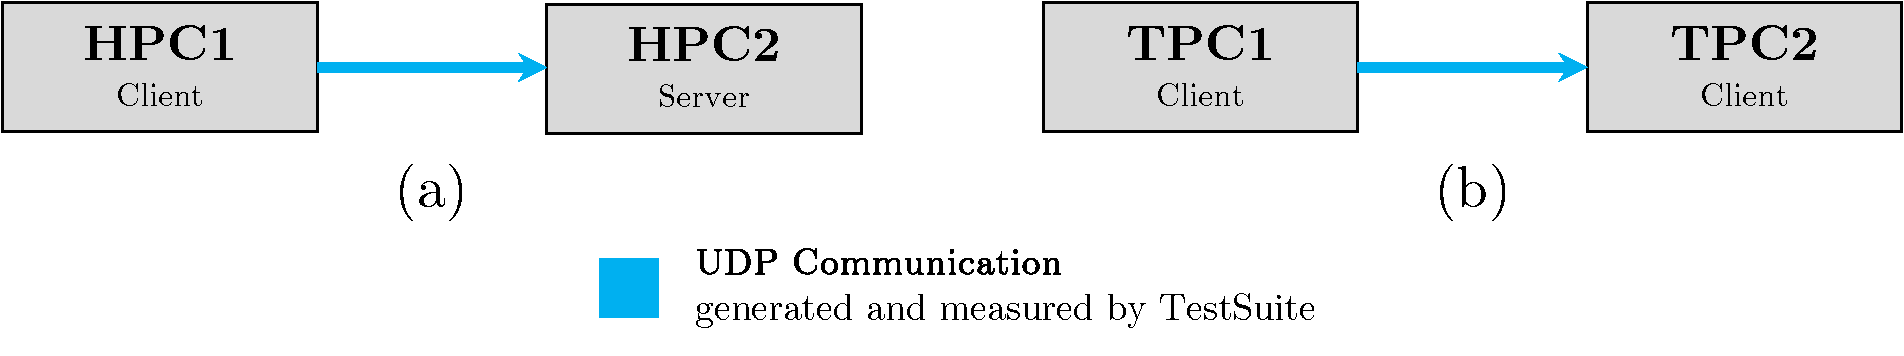
\includegraphics[width=1\linewidth]{figures/reliability/star/rel_g_1.pdf}
    \caption{Illustration of the used Systems under Test.}
    \label{fig:sutreliability}
\end{figure}

One system under test is a UDP communication generated by the Test Suite between the two High-Performance PCs (see Figure \ref{fig:sutreliability}a). HPC1, is the sender, also referred to as the client, and HPC2 is the receiver, also referred to as the server. Additionally, tests were conducted using the two Traffic PCs as the system under test (refer to Figure \ref{fig:sutreliability}b). The default settings of the network interfaces were used for all tests.

\subsection{Test Campaings}

\subsubsection{Isolated Tests in Different Operating States} \label{chap:relcamp1}
\paragraph{Motivation and Context}

As mentioned above, certain operating conditions can cause packet loss due to limited system resources. The purpose of this campaign is to identify the type of load on the test setup that causes packet loss. The following operating states are considered:

\begin{itemize}
  \item \textbf{System without any additional Load}
  \item \textbf{CPU Load} in User Space, Kernel Space and by Real-Time Processes (see \ref{chap:stressngCPU})
  \item \textbf{Memory Load} (see \ref{chap:stressngMemeory})
  \item \textbf{I/O Load} on internal Hard Disk (see \ref{chap:stressngIO})
  \item \textbf{Load due to Timer Interrupts} (see \ref{chap:stressngInterrupt})
  \item \textbf{Network Load} \\
  		Additional network load was generated with a participating computer system of the system under test. In the example of the High-Performance PCs as the SuT, this means UDP communication between the client or server and a Traffic PC. The Traffic PC is acting as the sender, and the respective computer system of the SuT is acting as the receiver.
  		
  \item \textbf{Traffic Load} \\
 		Traffic Load refers to bi-directional UDP communication between computer systems that are not part of the current system under test. The objective is to strain the switch.
\end{itemize}

The tools presented in \ref{chap:loadgeneration} are used to generate this load. The system is tested under maximum load. This means that as many stressors are used for the load generated with stress-ng as the system has logical CPU cores. A bandwidth of 10 GBit/s is used for the network stressors.

The presented operating states were tested individually for client and server. The two Traffic PCs as well as the High-Performance PCs were used as the system under test. The test duration for all tests was 100 seconds and a cycle time of 0 µs was used, whereby the maximum possible bandwidth was used for transmission. The datagram sizes used were 80 bytes as a representative for small datagrams in the test support system, 8900 bytes as a datagram size close to the MTU, and 65000 bytes as a datagram size close to the maximum of UDP.

\paragraph{Results}
In tests where the client was subjected to a generated load, no packet loss was detected in any of the tested operating states. This applies to both the tests with High-Performance PCs and Traffic PCs as a system under test.

\begin{figure}[h!]
  \centering
  \subcaptionbox{High-Performance PCs as System under Test\label{fig:resuc1a}}{%
    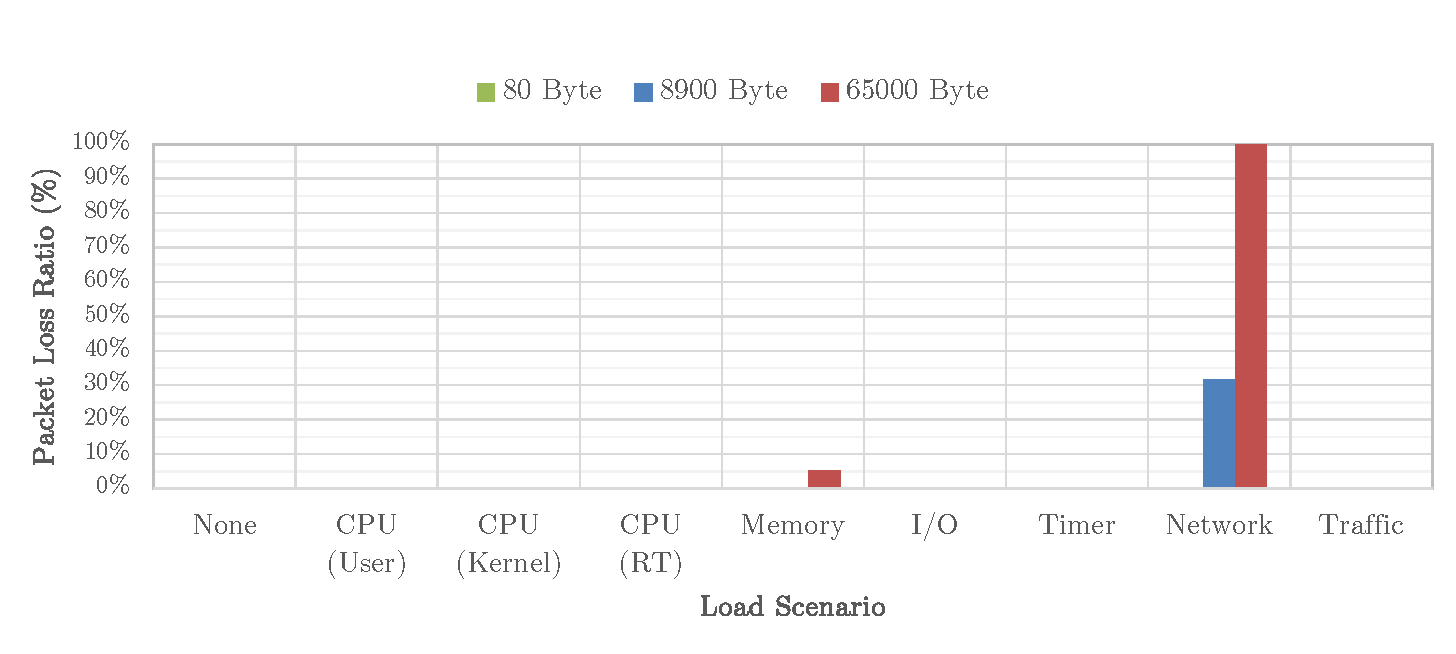
\includegraphics[width=1\textwidth]{figures/reliability/star/rel_d_1a.pdf}
  }
  \subcaptionbox{Traffic PCs as System under Test\label{fig:resuc1b}}{%
    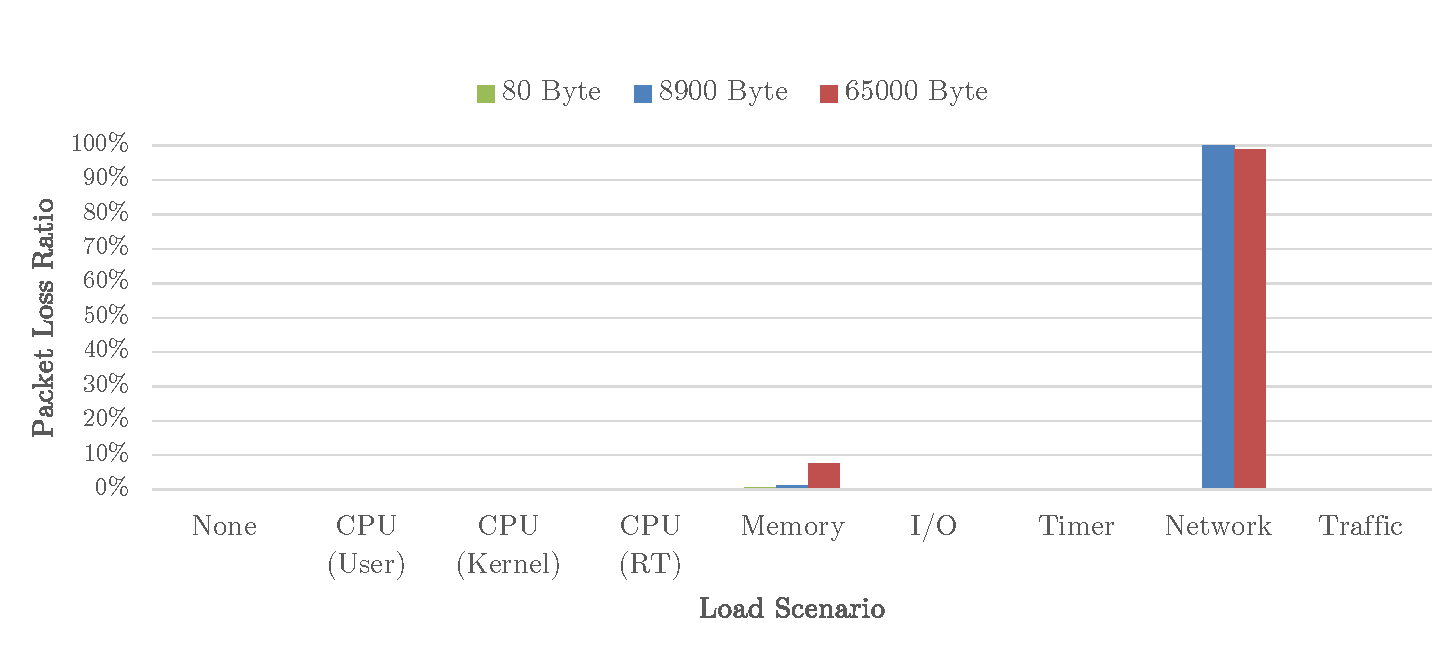
\includegraphics[width=1\textwidth]{figures/reliability/star/rel_d_1b.pdf}
  }
  \caption{Packet Loss Ratio for various Load Scenarios with different Datagram Sizes (Campaign `Isolated Tests in Different Operating States').}
  \label{fig:resuc1}
\end{figure}

During the stress tests where the server was subjected to a generated load, packet losses occurred on both systems under test. Figure \ref{fig:resuc1a} displays the percentage of packet losses in different load scenarios for High-Performance PCs, while Figure \label{fig:resuc1b} shows the results for Traffic PCs. The diagrams demonstrate that packet losses occurred in both systems under test when subjected to the stress-ng 'bigheap' stressor which generates memory load and to network load on the server.

Under stress from memory load, the server experiences packet losses across all three datagram sizes tested. Losses are less than one percent for 80 bytes and 8900 bytes, which is why they are not visible on the diagram. However, they increase to 5.29\% and 7.81\% for 65000 bytes, which is due to fragmentation, since the entire datagram is lost when a fragment is lost. It is also observed that the losses are slightly lower with the High-Performance PC as the system under test compared to the Traffic PC as the system under test when under memory load.

The losses occurred in the server, and the network card dropped the packets, as determined by the standard interface statistics of the network interface in the server. The drops occur due to memory load, as explained in \ref{chap:stressngMemeory}. This results in insufficient memory to process the arriving packets through the network stack. For instance, the network stack may not be able to allocate a socket buffer structure to process an incoming packet.

Additionally, packet losses have been observed with network load for datagram sizes of 8900 bytes and 65000 bytes. These are due to the maximum bandwidth being exceeded because both the client and another computer system are sending data to the server at up to 10 Gbit/s. As a result, the maximum bandwidth of 10 GBit/s, with which the server is connected to the switch, is exceeded, which is why packets get dropped by the switch.

\begin{figure}[htbp]
  \centering
  \subcaptionbox{Datagram Size of 80 Byte\label{fig:resuc2a}}{%
    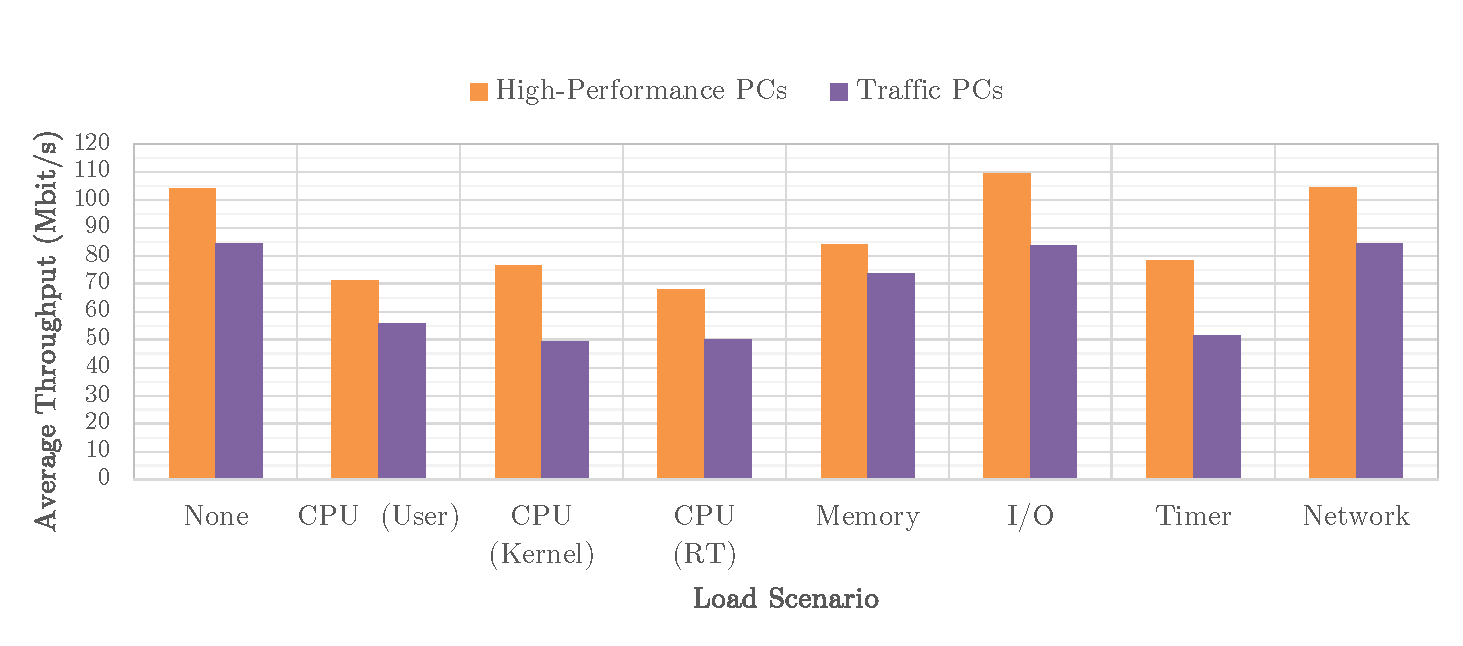
\includegraphics[width=0.9\textwidth]{figures/reliability/star/rel_d_2a.pdf}
  }
  \subcaptionbox{Datagram Size of 8900 Byte\label{fig:resuc2b}}{%
    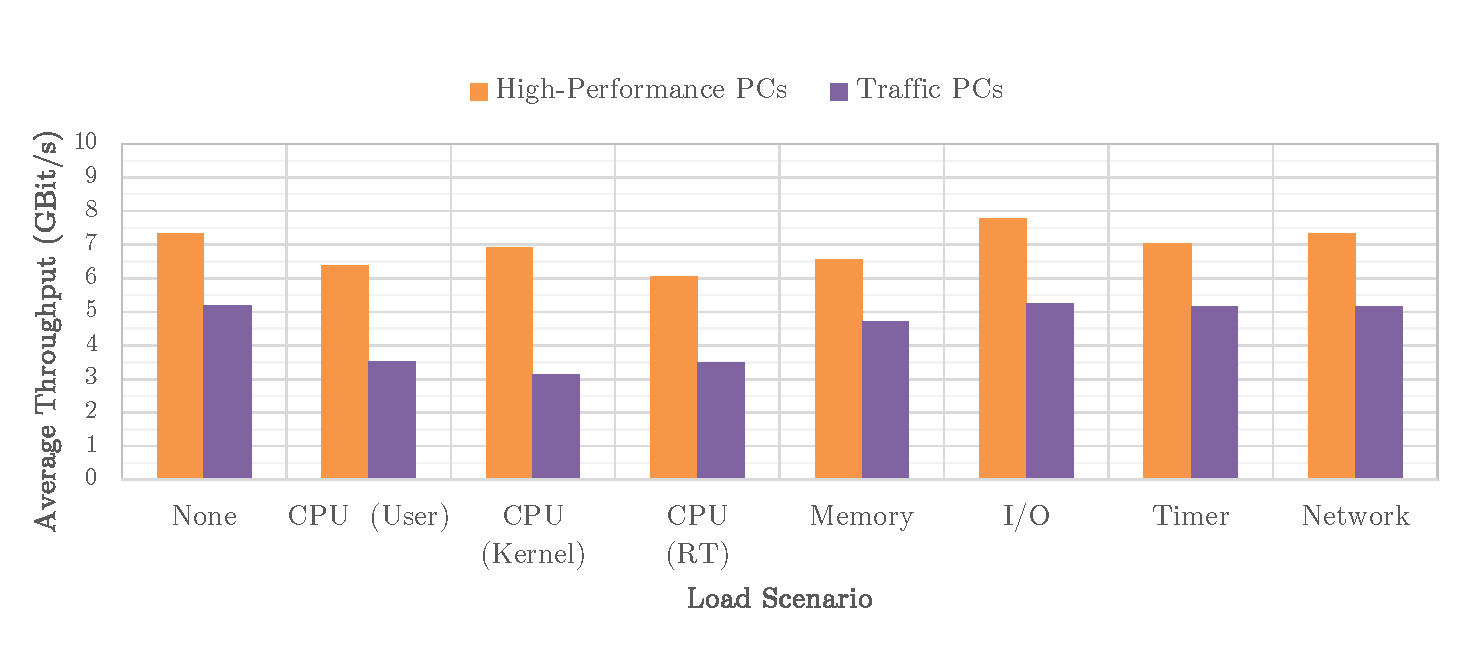
\includegraphics[width=0.9\textwidth]{figures/reliability/star/rel_d_2b.pdf}
  }
    \subcaptionbox{Datagram Size of 65000 Byte\label{fig:resuc2c}}{%
    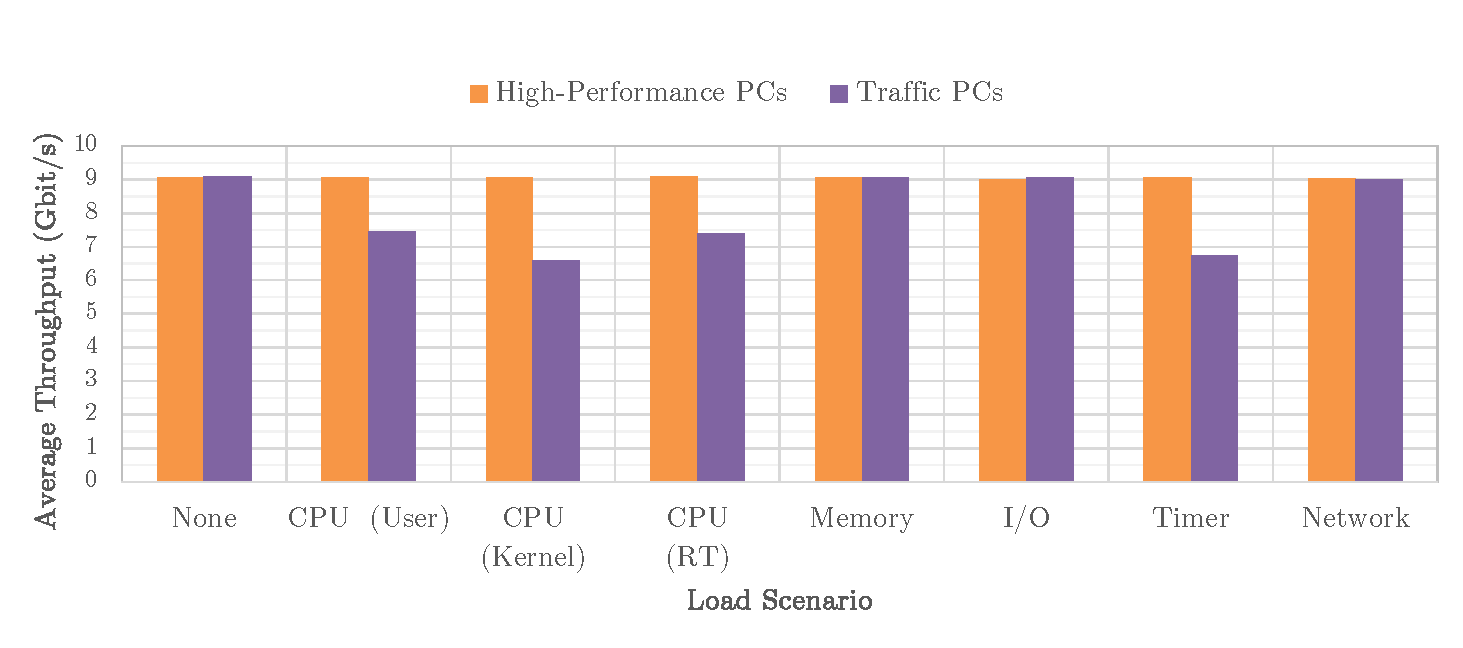
\includegraphics[width=0.9\textwidth]{figures/reliability/star/rel_d_2c.pdf}
  }
  \caption{Average Throughput for various Load Scenarios (Campaign `Isolated Tests in Different Operating States').}
  \label{fig:resuc2}
\end{figure}

As mentioned above, there were no packet losses during the tests where the client was loaded. However, the stress did affect the average throughput sent to the server. Figure \ref{fig:resuc2} compares the average throughput of the High-Performance PCs and Traffic PCs as system under test in different operating conditions.

On one side, the average throughput of the High-Performance PCs is higher than that of the Traffic PCs, especially for datagram sizes of 80 bytes and 8900 bytes. All categories of CPU load, memory load, and load due to timer interrupts have a negative impact on the average throughput, with a reduction of 5\% to 10\% greater for Traffic PCs than for High-Performance PCs, particularly for datagram sizes of 80 bytes and 8900 bytes.  At 65,000 bytes, the throughput of High-Performance PCs remains unaffected by any stress, while the throughput of Traffic PCs is reduced by up to 25\% by CPU and timer interrupt load.

These differences in average throughput and the impact of additional system load on it are due to differences in hardware. The hardware of High-Performance PCs is significantly more powerful than that of Traffic PCs (see \ref{chap:ComputerHardware}), which enables them to transmit a larger number of packets.

\paragraph{Classification of Results}
The campaign found that the reliability of the server can be negatively impacted by the memory load and network load operating states. However, it is important to note that these isolated operating conditions are not realistic.

A system that constantly suffers from a memory overload, as caused by the memory load scenario, is a conceptual error because too less memory is installed.

Regarding the examined network load scenario, it is logical to discard packets if the maximum bandwidth is exceeded. However, it should be noted that this situation can occur in asynchronous systems, such as a Distributed Test Support System.

\subsubsection{Tests with Realistic Load Scenario} \label{chap:campaignloadscen}
\paragraph{Motivation and Context}
In the previous campaign (refer to \ref{chap:relcamp1}), individual operating states were considered in isolation. The highest possible load was always taken into account, but this does not correspond to the typical load in a Distributed Test Support System.

{
\renewcommand{\arraystretch}{1.3}

\begin{table}[h]
\centering
\newcolumntype{C}[1]{>{\raggedright\arraybackslash}p{#1}}

\begin{tabularx}{\textwidth}{C{8cm} | l | X}
	\toprule
	\textbf{Load Component} & \textbf{Quantity} & \textbf{Analogy}\\
	\midrule
	Real-Time Process with 100\% CPU Utilization & 4 & Simulations\\
	Real-Time Process with 5\% CPU Utilization & 20 & Global Memories\\
	Process with I/O Load on internal Disk with Data Rate limited to 1 GBit/s & 1 & Data Logging\\
	Timer with a Frequency of 100 kHz & 1 & \\
	\bottomrule
\end{tabularx}

\caption{Components of the Realistic Load Scenario for a Computer System.}
\label{tab:realpc}
\end{table}
}

\vspace{20pt}

\begin{figure}[h!]
    \centering
    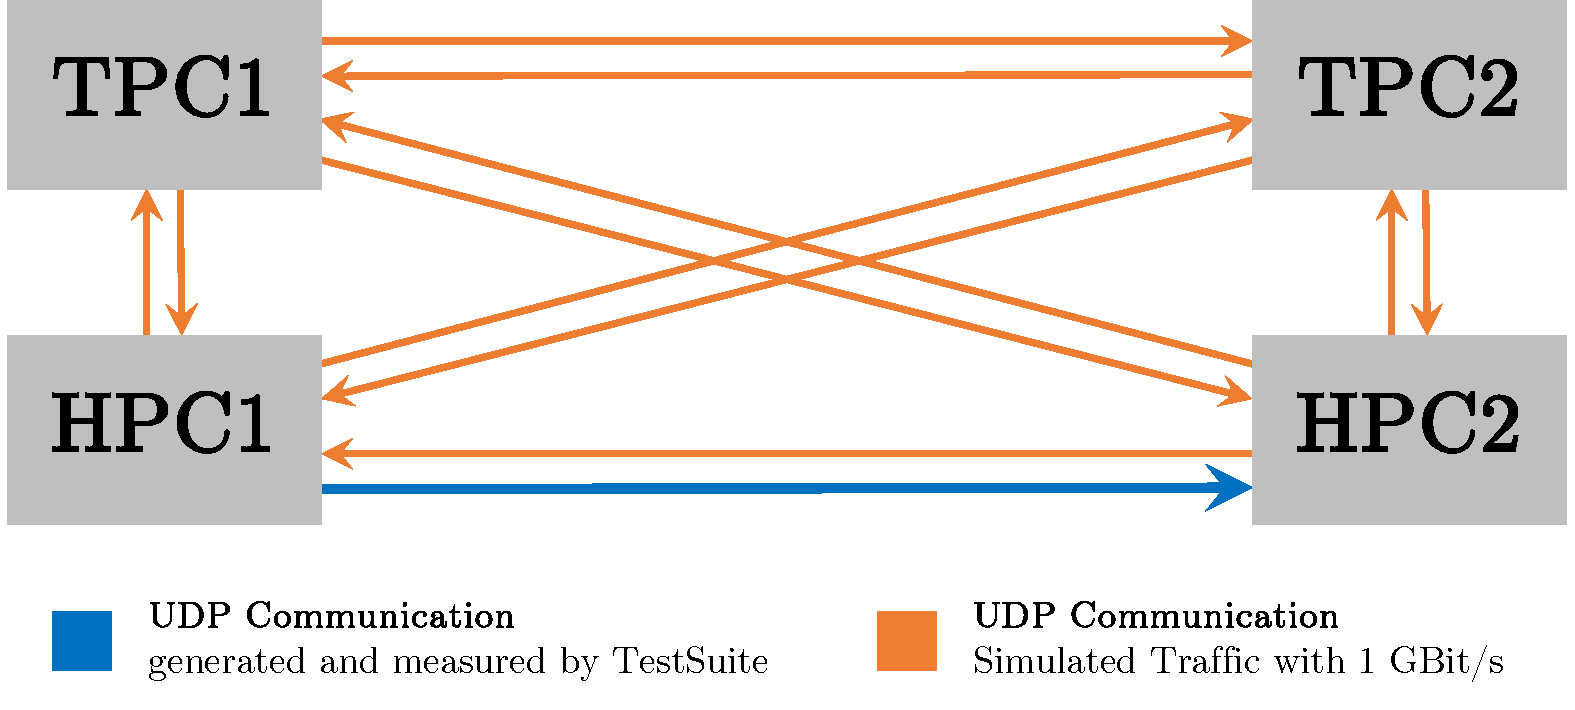
\includegraphics[width=0.8\linewidth]{figures/reliability/star/rel_g_2.pdf}
    \caption{Representation of the Network Load in the Realistic Load Scenario.}
    \label{fig:realNW}
\end{figure}

Therefore, a realistic load scenario has been developed based on practical experience with a Distributed Test Support System, which includes the load on the computer systems as well as on the network. Table \ref{tab:realpc} contains the components of this scenario, which is executed on all computer systems, as well as their analogy in a real Distributed Test Support System. These components are generated using stress-ng. Furthermore, the realistic scenario involves UDP network traffic generated with iPerf between all four computer systems of the topology, with a bandwidth limitation of 1 GBit/s per channel, excluding the communication generated and measured by the TestSuite. Figure \ref{fig:realNW} illustrates this, with an example of the High-Performance PCs as the system under test.

This scenario generates a CPU utilization of 56.9\% on a High-Performance PCs without running a test. On a Traffic PCs, the scenario generates a much higher CPU utilization of 100\%, which means the system is fully utilized.

The objective of this campaign is to assess the reliability of the setup under this load. Similar to the previous campaign, datagram sizes of 80 bytes, 8900 bytes, and 65000 bytes will be considered. Additionally, the query function of the TestSuite described in \label{chap:targetcom:query} is used for these tests. A test will be terminated if more than 50 datagram losses occur, as this is considered to be an unreliable communication. The maximum duration of the test is 2 hours.

To examine various bandwidths, the cycle time is systematically increased as well. Starting with an initial value of 0 µs for all datagram sizes, the cycle time is increased in steps of 10 µs. For datagram sizes of 65,000 bytes, the increase starts at a cycle time of 60 µs. This is because, as shown in table \ref{tab:senditertime}, a run through the send loop takes more than 60 µs on average. Testing shorter cycle times would therefore not provide any further insight. The objective of varying the cycle time is to determine the maximum bandwidth possible without experiencing packet loss.

\paragraph{Results}
The campaign was performed with both the High-Performance PCs and the Traffic PCs as the system under test. Although the results differ in absolute terms, they yield the same findings. Therefore, only the results of the High-Performance PCs will be discussed below.

\begin{figure}[h!]
  \centering
  \subcaptionbox{Datagram Size of 8900 Byte\label{fig:resuc3a}}{%
    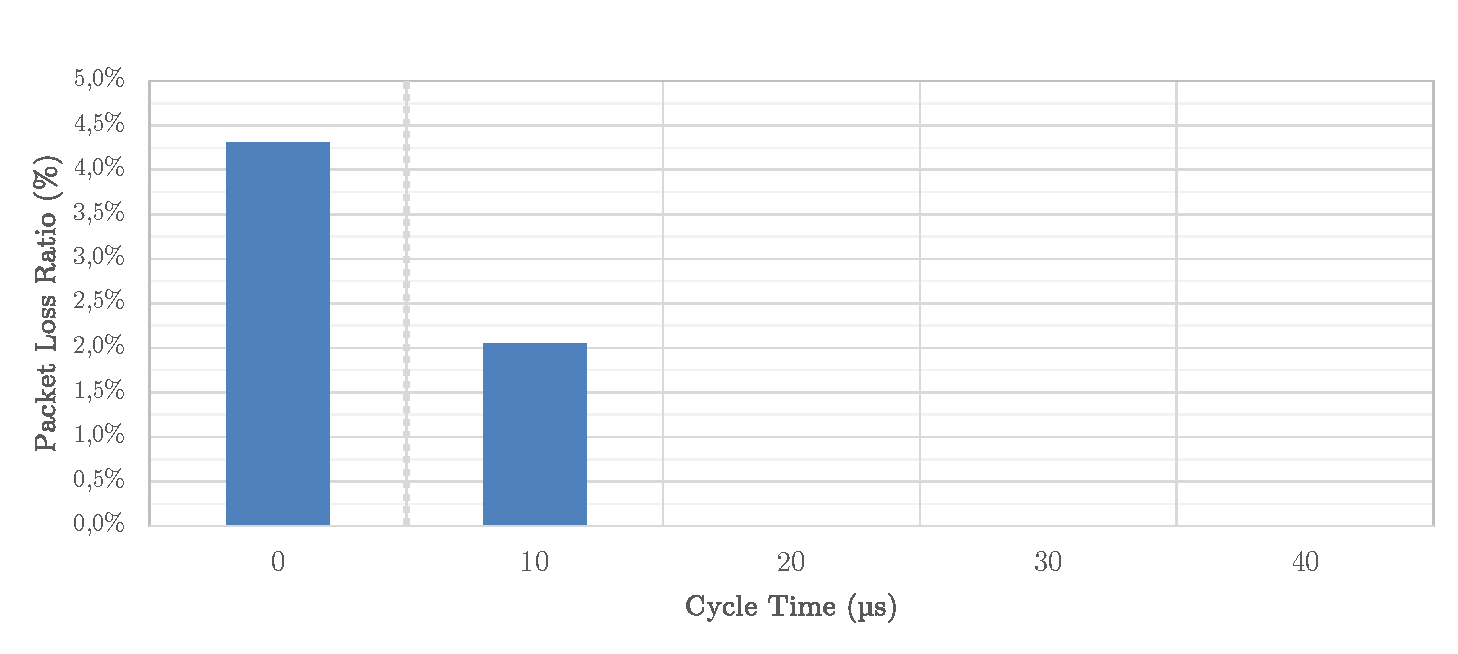
\includegraphics[width=1\textwidth]{figures/reliability/star/rel_d_3a.pdf}
  }
  \subcaptionbox{Datagram Size of 65000 Byte\label{fig:resuc3b}}{%
    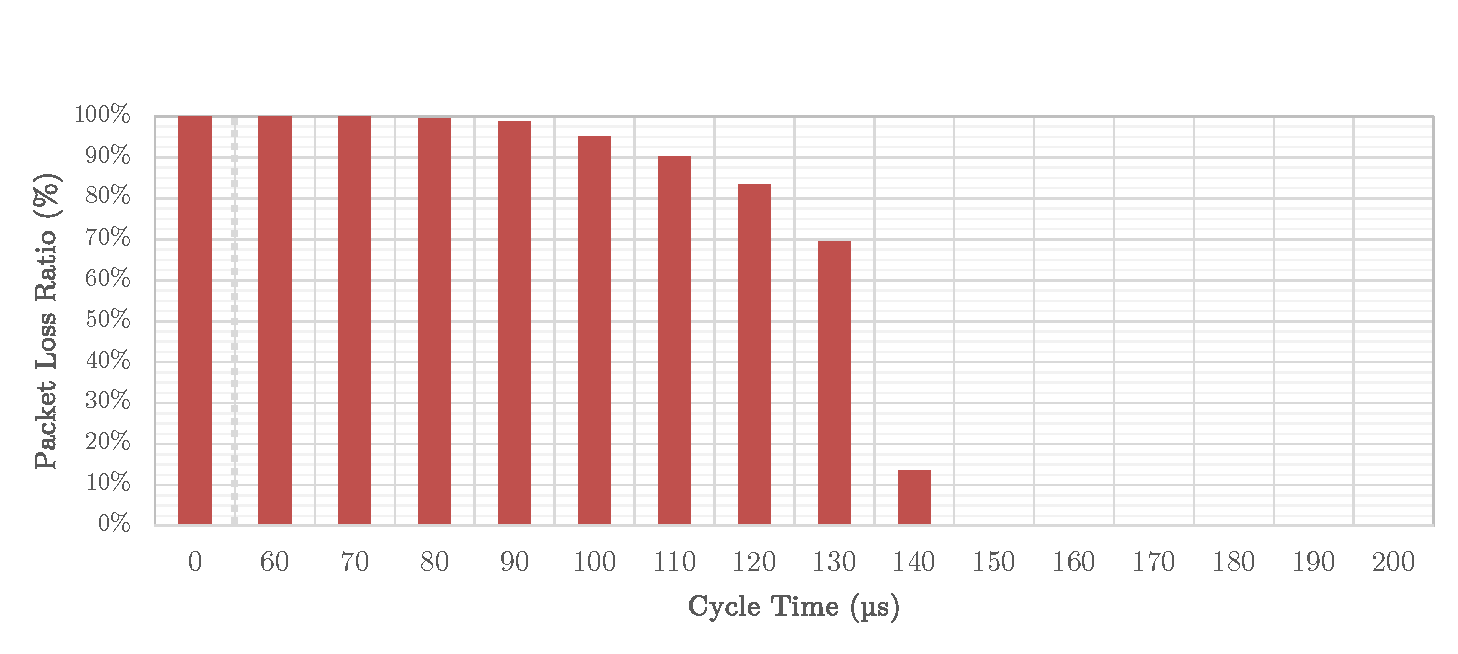
\includegraphics[width=1\textwidth]{figures/reliability/star/rel_d_3b.pdf}
  }
  \caption{Packet Loss Ratio by Cycle Time with High-Performance PCs as System under Test (Campaign `Tests with Realistic Load Scenario').}
  \label{fig:resuc3}
\end{figure}

Figure \ref{fig:resuc3} displays the percentage of packet losses for various cycle times in tests conducted on High-Performance PCs as a system under test. Results are shown for a datagram size of 8900 bytes in \ref{fig:resuc3a} and 65000 bytes in \ref{fig:resuc3b}. No Loses were detected in tests with a datagram size of 80 bytes.

For a datagram size of 8900 bytes, packet losses were detected at cycle times ranging from 0 µs to 30 µs. Notably, significant packet losses of 4.31\% and 2.05\% occurred at 0 µs and 10 µs, respectively, while only isolated losses were observed at 20 µs and 30 µs. For datagrams with a size of 65000 bytes, significantly higher losses were observed. Over 90\% of packet loss occurred up to a cycle time of 110 µs, after which the percentage of packet loss decreases. No losses occurred starting at a cycle time of 210 µs.

The statistics recorded in the examined computer systems (Standard Interface Statistic and Network Stack Statistic) do not indicate any packet drops, so the sender and receiver can be excluded as the source of the loss.

This turns the switch into a possible source of packet loss. The switch has statistics called 'Tail Drops' that can be viewed for each port in the switch's web interface. These reflect the drops that occur when the output queue of a port is full. The switch will discard data until the output queue is cleared again \cite {reli02}. These described drops occurred during the execution of the tests.

For cycle times of 0 µs and 60 µs with a datagram size of 65000 bytes, the losses can be explained by the possible exceeding of the maximum bandwidth of 10 GBit/s. The average throughput in the tests was 9.0 GBit/s and 8.3 GBit/s, which, in combination with the network load in the realistic scenario (2 GBit/s of incoming traffic on HPC2), operates at the maximum bandwidth with which HPC2 is connected to the switch. However, with a 100 µs cycle time, for example, the average throughput is only 5.2 GBit/s, which means that even in combination with the realistic scenario, the maximum bandwidth is not reached. This also applies to packet losses with a datagram size of 8900 bytes.

At 65000 bytes, exceptionally high losses also occur at cycle times of up to 140 µs, even if the available bandwidth is not exceeded, as explained above with 100 µs as an example. Fragmentation may be one reason for this phenomenon of the high losses, since the entire datagram is discarded when a fragment is lost.

In order to better understand the packet losses, certain tests were repeated and the results of the query requests were recorded. This allows the analysis of the temporal occurrence of packet losses.

\begin{figure}[h!]
    \centering
    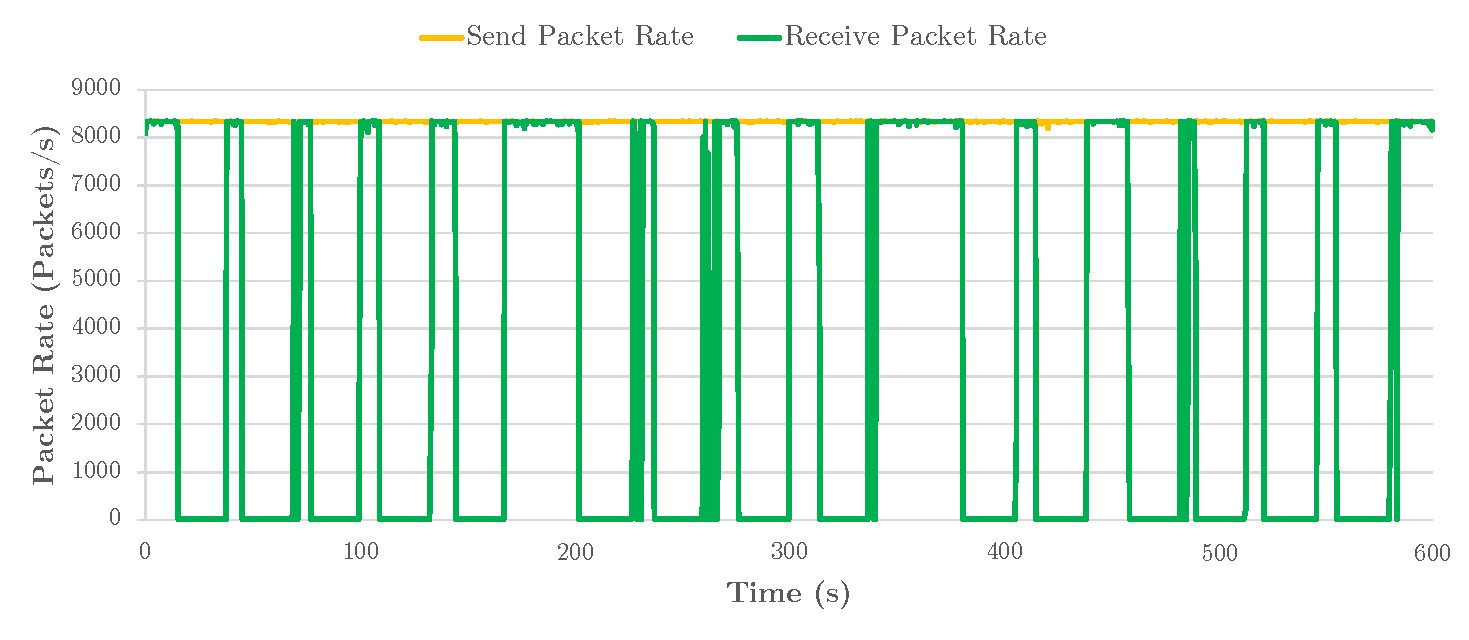
\includegraphics[width=1\linewidth]{figures/reliability/star/rel_d_4.pdf}
    \caption{Sent and Receive Packet Rate over Time for a Test with a Datagram Size of 65000 Byte and a Cycle Time of 120 µs (Campaign `Tests with Realistic Load Scenario').}
    \label{fig:srpr4}
\end{figure}

Figure \ref{fig:srpr4} displays the send and receive packet rate over time for an example test with a datagram size of 65000 bytes and a cycle time of 120 µs. The average throughput was 4.3 Gbit/s, and there was a 61\% packet loss. The variation in packet losses between this implementation and the results presented in \ref{fig:resuc3} for a cycle time of 120 µs can be attributed to fluctuations.

The diagram shows that the packet losses occur cyclically. It is illustrated that there are phases during which all packets are lost and phases during which nearly all packets are received. These phases of packet loss have a constant duration of 25 seconds, but the interval between these phases varies.

Based on recorded data, it can be concluded that the packet losses occurred due to an overload the switch. The recorded pattern with the constant loss intervals could indicate an kind of overload protection mechanism of the switch, which prevents the sending of packets. However, the Ethernet switch is a 'Black Box', as Cisco does not publish detailed information about the implementation, so the exact cause of the losses cannot be analyzed further. During the tests, all protection mechanisms of this kind, which can be set in the switch interface, were deactivated.

\paragraph{Classification of Results}
This campaign showed that packet losses can occur when the setup is loaded with the realistic scenario. Losses were also observed below the maximum bandwidth. The reason for this is most likely due to switch congestion, which occurs cyclically.

\subsubsection{Tests with Realistic Load Scenario and Quality of Service}
\paragraph{Motivation and Context}
This test campaign examines the impact of using Quality of Service on the result. The IP header's Differentiated Services field is utilized for this purpose. The TestSuite specifies a priority of 63 for its communication, which is the highest possible value. The switch is also configured to prioritize packets with this priority.

The realistic scenario is executed on all systems involved in the setup, as in the previous campaign. The network traffic generated as part of the scenario is not given preferential treatment by the switch, as no priority is assigned to it.

The test procedure selected for this campaign is the same as the one used for the 'Tests with Realistic Load Scenario' campaign (see \ref{chap:campaignloadscen}). Datagram sizes of 80 bytes, 8900 bytes, and 65000 bytes were taken into consideration. The system under test includes both the High-Performance PCs and the Traffic PCs.

The test campaign examined not only the Intel X710-T2L network interfaces that are the default for the topology, but also the Intel X540-T2, the Inspur X540-T2 and the Lenovo QL41134, which were tested with the High-Performance PCs as the system under test.

\paragraph{Results}
In tests with the High-Performance PCs, no packet loss was detected for all datagram sizes tested, with the smallest cycle time tested of 0 µs for 80, 8900, and 65000 bytes. The average throughput achieved in these tests was 91.5 MBit/s for 80 bytes, 7.23 GBit/s for 8900 bytes, and 9.01 GBit/s for 65000 bytes. There were no packet losses in the tests with the alternative network cards (Intel X540-T2, Inspur X540-T2 and Lenovo QL41134). The achieved average throughput in these tests is similar to that of the Intel X710-T2L.

Also, no packet loss was detected in the tests with the Traffic PCs with the shortest cycle time. The average throughputs were 52.1 MBit/s for 80 bytes, 4.88 GBit/s for 8900 bytes, and 7.41 GBit/s for 65000 bytes. This also shows that, as mentioned in the first campaign (see \label{chap:relcamp1}), the system load of the traffic PCs has a greater influence on the average throughput achieved by the sender.

However, packet losses were detected in all tests for the traffic generated by iPerf in the context of the realistic load scenario. These effects were caused by the switch, as shown by its statistics.

\paragraph{Classification of Results}
The campaign has demonstrated that reliability can be ensured through the use of quality of service. However, this requires traffic to be prioritized. Nevertheless, packet losses were detected in non-prioritized traffic. Currently, the Distributed Test Support System does not provide such prioritization, so no QoS can be applied.

Another finding from this campaign is that the two computer systems in the system under test (client and server) do not cause any packet losses even when under stress from the realistic scenario. This confirms the assumption made in the previous campaign 'Tests with Realistic Load Scenario' based on the recorded statistics.

Furthermore, the campaign has shown that the Intel X540-T2, Inspur X540-T2 and Lenovo QL41134 network interfaces have comparable reliability to the Intel X710-T2L.

\subsubsection{Tests with Realistic Load Scenario and Custom Network Load Generator}
\paragraph{Motivation and Context}
The `Tests with Realistic Load Scenario' campaign (see \ref{chap:campaignloadscen}) has already concluded that the switch suffered from an overload situation. The purpose of this campaign is to further analyze the circumstances that led to packet loss in the switch.

One possible reason for the occurrence of packet losses through the switch is the bursts sent by the network traffic generated by iPerf for the realistic scenario, which cause a short-term overload of the switch. This assumption is supported by the observation that packet losses occur in the switch when executing the realistic scenario in the test setup, even without running a test campaign. Due to the specified bandwidth of 1 GBit/s per channel in the realistic scenario, it is expected that no packet losses will occur as the network's maximum bandwidth is significantly higher.

iPerf utilizes a throttling algorithm to regulate the specified bandwidth. This algorithm monitors the data throughput sent at 100 ms intervals and adjusts it as needed to maintain specified bandwidth \cite{reli03}. Unlike CPU stressors, which run as real-time processes in a realistic load scenario, iPerf is not executed as a real-time process on the system. This can result in iPerf not being allocated sufficient computing time. As a result, the throttling algorithm may make extreme adjustments to achieve the required bandwidth, which may result in data bursts being sent. However, it is not possible to verify this assumption by recording with Wireshark due to hardware limitations.

In this test campaign, a self-programmed network traffic generator based on TestSuite replaces iPerf in the realistic load scenario. Unlike iPerf, this generator does not use a throttling algorithm and therefore does not send any bursts. Furthermore, the process is executed in real-time with a priority of 90, which is higher than that of the stressors but lower than that of TestSuite. The cycle time was configured to ensure a maximum transmission bandwidth of 1 GBit/s.

The test procedure for this campaign was the same as for the 'Tests with Realistic Load Scenario' campaign (see \ref{chap:campaignloadscen}). Datagram sizes of 80 bytes, 8900 bytes, and 65000 bytes were considered. Tests were performed exclusively with the High-Performance PCs as the system under test. Quality of Service was not utilized.

\paragraph{Results}

\begin{figure}[h!]
    \centering
    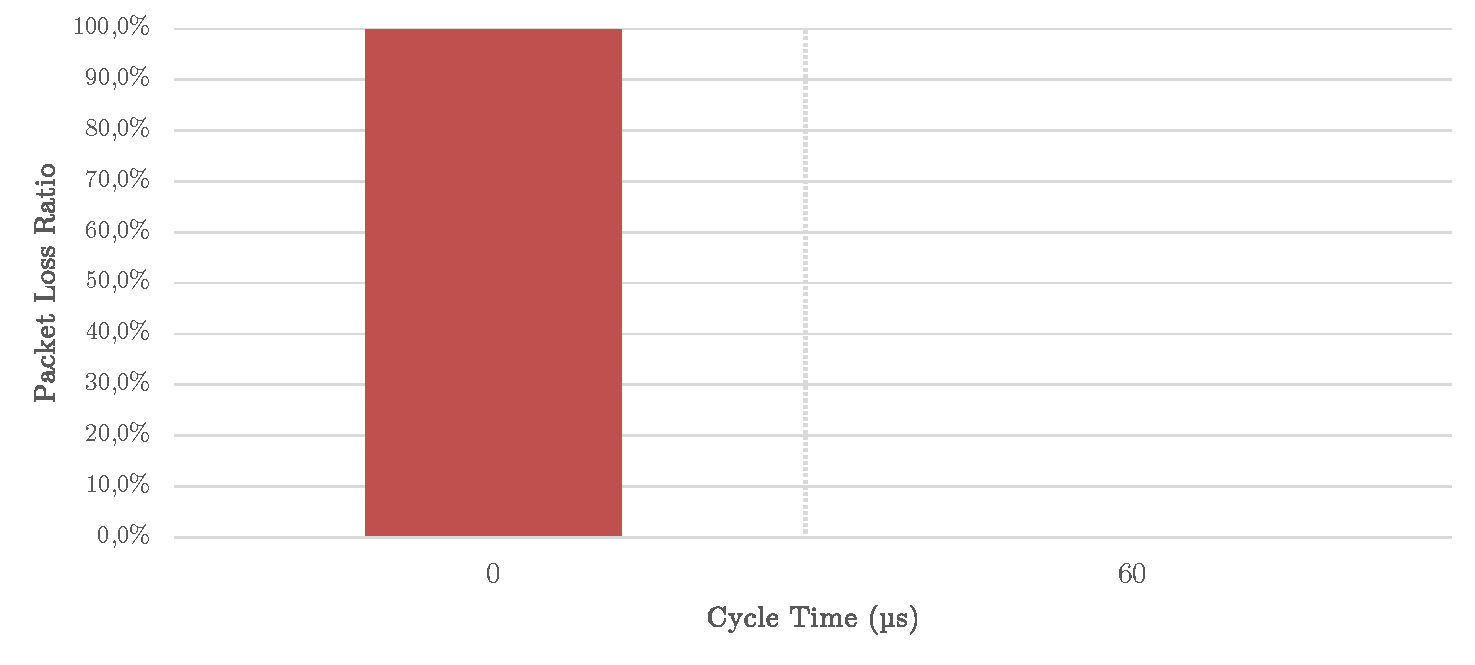
\includegraphics[width=1\linewidth]{figures/reliability/star/rel_d_5.pdf}
    \caption{Packet Loss Ratio by Cycle Time for a Datagram Size of 65000 Byte with High-Performance PCs as System under Test (Campaign `Tests with Realistic Load Scenario and Custom Network Load Generator').}    \label{fig:srpr5}
\end{figure}

During the campaign, only packet losses were observed when examining a datagram size of 65000 bytes. At a cycle time of 0 µs, packet losses of 99.9\% were recorded. while no packet losses occurred at a cycle time of 60 µs. These results are illustrated in Figure \ref{fig:srpr5}. It is worth noting that packet drops were again only reported by the switch.

A major reason for the high number of packet losses at 65000 byte datagram size and 0 µs cycle time is the fact that the maximum bandwidth of 10 Gbps is exceeded, as the average throughput in the test is 9.1 Gbps. Additionally, packet loss is increased by the use of fragmentation.

\paragraph{Classification of Results}
Compared to using iPerf (see \ref{chap:campaignloadscen}), a separate network stressor significantly reduces packet losses. This suggests that iPerf generates bursts that overload the switch and cause packet loss. However, it should be noted that the systems in the Distributed test support system are asynchronous, meaning they can also send out bursts that should not overload the network.

\subsection{Insights}
The investigation of the star topology with a switch in the center has revealed that an Ethernet switch is unsuitable for use in the Distributed Test Support System. The switch was found to be the cause of packet loss, particularly in connection with burst traffic.

Another concern is that the maximum bandwidth at which each participant is connected to the switch may be exceeded. Since the Distributed Test Support System is an arrangement of independent systems, such an exceedance cannot be excluded.

Regarding the computer systems, the investigation showed that a memory load that provokes a constant memory overflow can lead to packet loss. However, it was also found that both High-Performance PC and Traffic PC systems do not experience packet losses when subjected to a load similar to that in a real Test Support System.

Furthermore, in addition to the standard network interfaces in the topology, the Intel X540-T2, Inspur X540-T2, and Lenovo QL41134 network interfaces were also examined, and no reduction in reliability based on packet loss was found, making them equally suitable for use in a Distributed Test Support System.




\section{Reliability Analysis of the Star Topology with the iHawk in the Centre} \label{chap:ReliabIhawk}

\subsection{System under Test} \label{chap:ReliabIhawk:SuT}
The key takeaway from the previous reliability tests (see \ref{chap:switchtest}) is that the use of an Ethernet switch in the Distributed Test Support System is unsuitable, as it leads to a significant number of lost packets. Additionally, the behavior of the switch was found to be unreliable and unpredictable. As a result, an alternative topology was developed and investigated, which is described in \ref{chap:TopoiHawk}, and in which the iHawk is placed in the center of the star.

In this configuration, all participants (hereafter referred to as Endpoints) are connected to a computer system in the center (hereafter referred to as the Center). In a practical implementation in the test system, the endpoints are the I/O PCs and the center is an iHawk. The endpoints are not connected to each other, as communication in the Distributed Test Support System is mainly between the center and the endpoints, rather than between the endpoints themselves.

For the test setup, the High-Performance PCs and Traffic PCs serve as endpoints, while an iHawk is located in the center. Unless otherwise specified, the network cards mentioned in the presenation of the topology (see \ref{chap:TopoiHawk}) will be used for the tests.

The system under test for subsequent test campaigns is no longer a single communication that is examined. Instead, the TestSuite examines each bidirectional link in the topology. Since each of the four endpoints is connected to the center by two bidirectional links, there are 16 UDP communications generated and measured by the TestSuite.

\begin{figure}[h!]
    \centering
    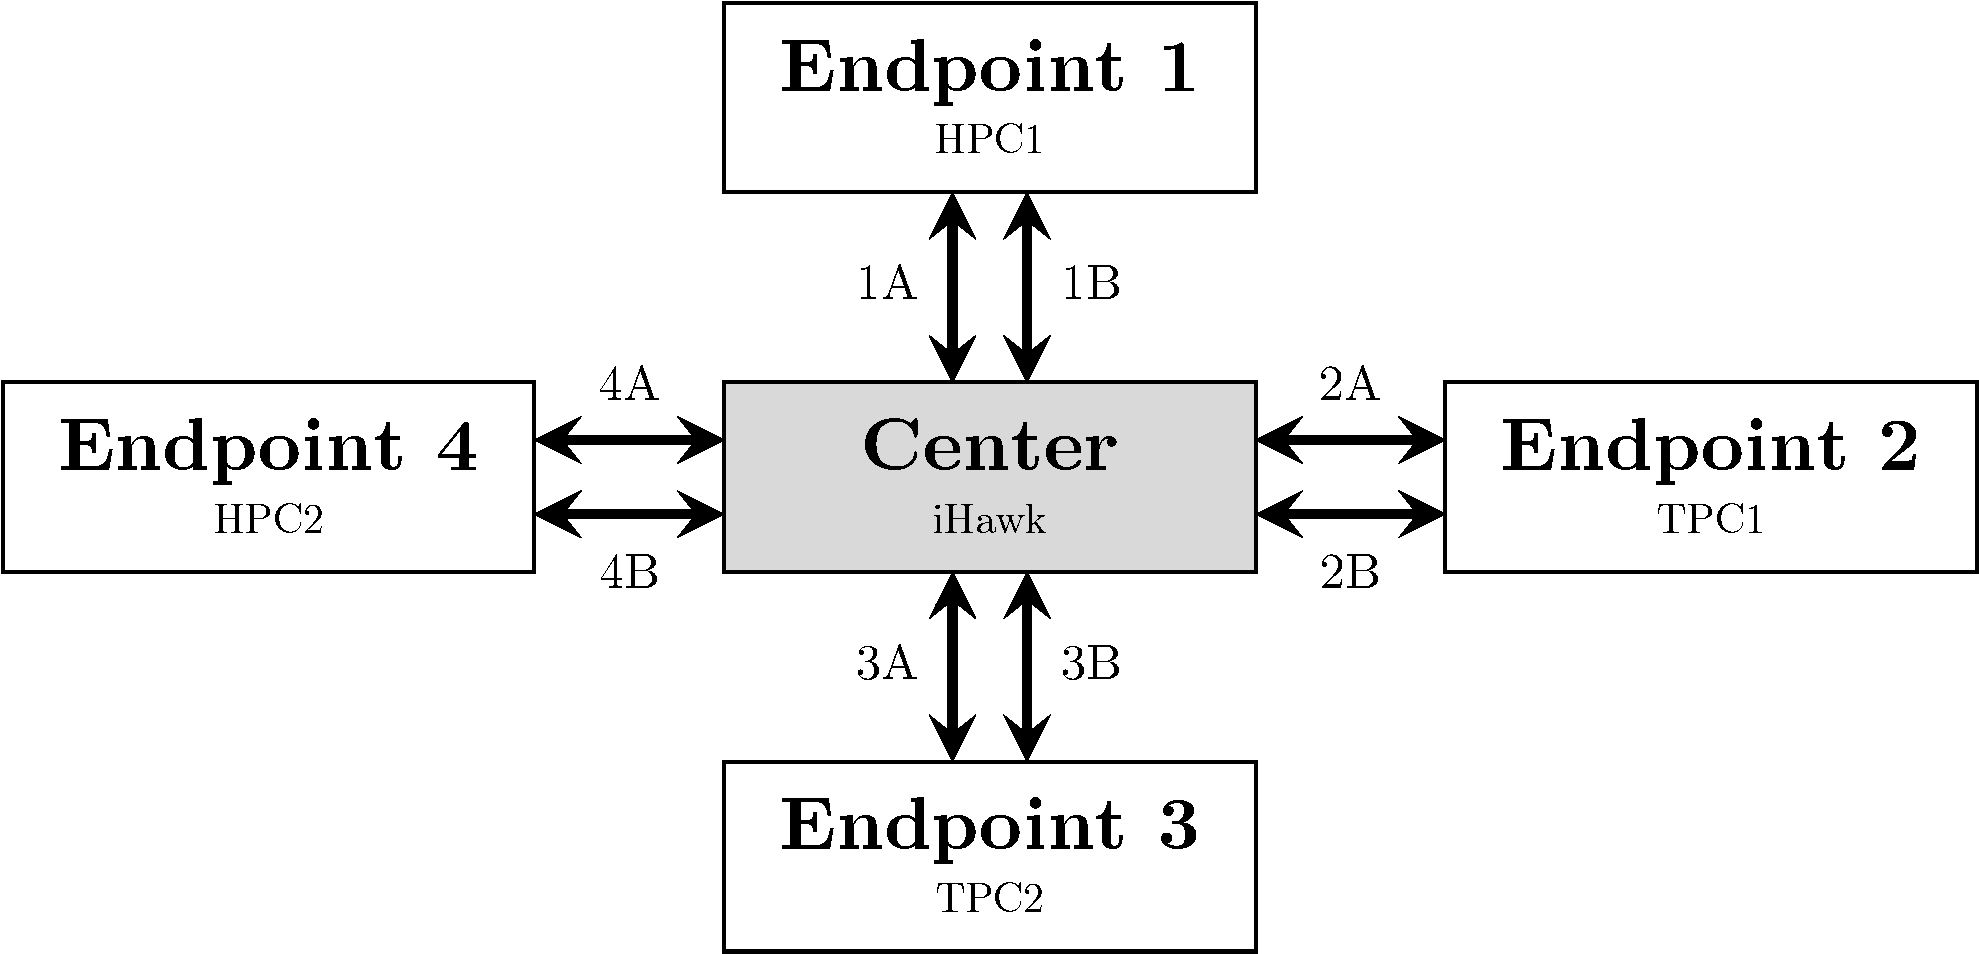
\includegraphics[width=0.8\linewidth]{figures/reliability/ihawk/topo.pdf}
    \caption{Structure and Nomenclature of Communication Channels of the Test Setup with the iHawk in the Center of the Star.}
    \label{fig:topoihawknaming}
\end{figure}

To distinguish between communications more easily, the nomenclature scheme depicted in Figure \ref{fig:topoihawknaming} was designed. The two physical 10 GbE links that connect each endpoint to the centers are referred to as link `\textbf{A}' and `\textbf{B}'. A separate TestSuite process generates and measures UDP communication in both directions across each of these links simultaneously. These directions are referred to as `\textbf{H}' and `\textbf{R}'. Direction `H' refers to communication channels where the center is the sender and the endpoint is the receiver. Conversely, direction `R' refers to communication channels where the center is the receiver and the endpoint is the sender.

Because 16 bidirectional communications lead to a high network load, especially in the center, the settings recommended by Intel for high performance and reliability in the Linux Performance Tuning Guide for the Ethernet 700 Series \cite{intermod03} were used. These settings were chosen based on experiments conducted with the High-Performance PCs prior to this campaign. These settings include:
\begin{itemize}
  \item Disabling of Energy Efficient Ethernet
  \item Enlargement of the RX\_Ring and TX\_Ring to 4096 slots
  \item Deactivation of Interrupt Moderation (unless otherwise specified)
  \item UDP Receive Buffer Size of 25 MB
\end{itemize}

\subsection{Test Campaigns}

\subsubsection{Tests without additional Load} \label{chap:noaddloadTest}
\paragraph{Motivation and Context}
This test campaign aims to assess the reliability of the setup when all 16 communication channels are operating at full capacity. The center, which has to handle a high communication load, is the main focus of the campaign.

To analyze the reliability in a long-term test, a test duration of 2 hours is used. Datagram sizes of 80 bytes, 8900 bytes and 65000 bytes are tested and a cycle time of 0 µs is selected, which corresponds to an uninterrupted transmission process.

\paragraph{Results}
\subparagraph{System Utilization}
Before presenting the results on reliability based on the number of packet losses, this section discusses the utilization of the systems, especially the utilization of the iHawk in the center.

\begin{figure}[h!]
    \centering
    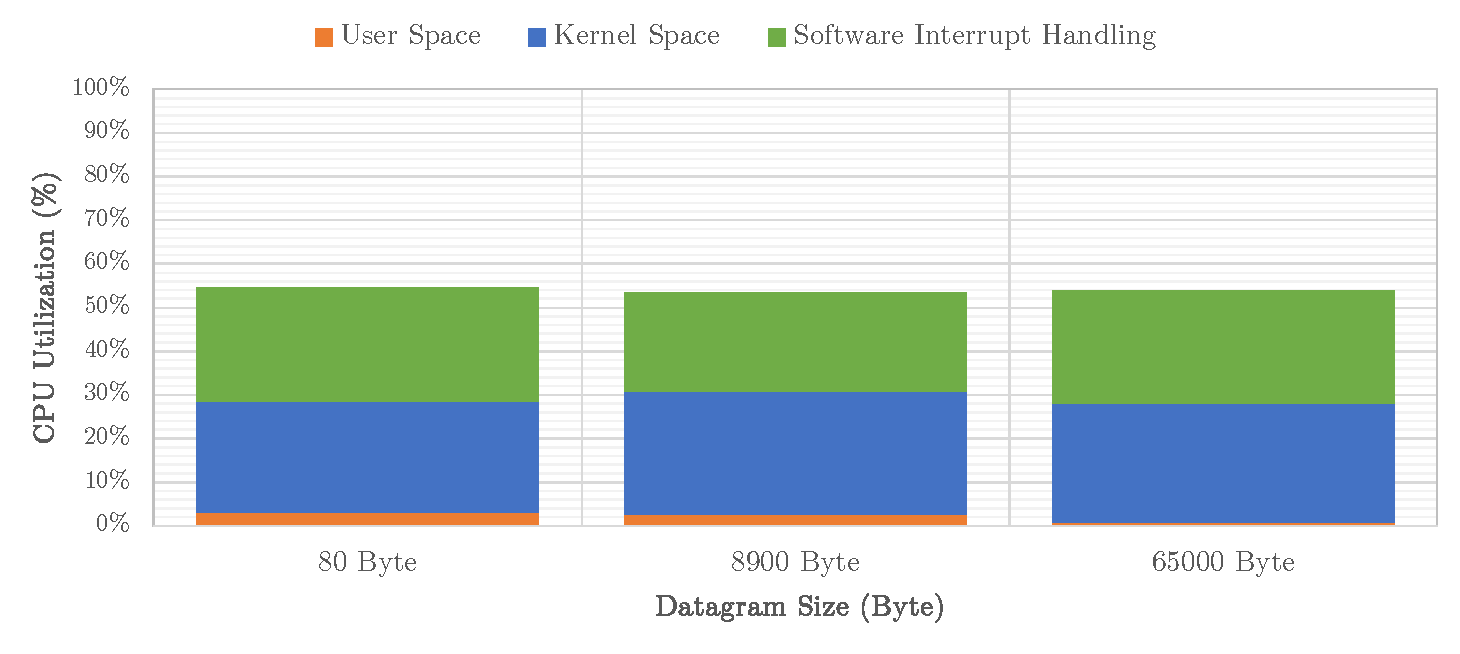
\includegraphics[width=1\linewidth]{figures/reliability/ihawk/diagr2.pdf}
    \caption{CPU Utilization in the Center for the examined Datagram Sizes (Campaign `Tests without additional Load').}
    \label{fig:diagr2CPU}
\end{figure}

Figure \ref{fig:diagr2CPU} displays the average CPU utilization at the center for the examined datagram sizes. The overall utilization across all datagram sizes is about 55\% and varies slightly. As the datagram size increased, the utilization in the user space decreased while the utilization in the kernel space increased. Additionally, utilization was also observed in the software interrupt handling area.

The increased user space utilization, especially for datagrams with a size of 80 bytes, is due to the higher number of packets generated or retrieved in the application (TestSuite). While about 100,000 packets per second are processed with an 80 byte datagram size, only about 19,000 packets per second are processed with a 65,000 byte datagram size.

The utilization in the software interrupt handling area includes packet processing during reception and partially during transmission. The lowest utilization is measured with a datagram size of 8900 bytes, because fewer packets are processed (compared to 80 bytes) and no fragmentation or defragmentation is performed (compared to 65000 bytes).

The CPU utilization was monitored throughout the testing period and no anomalies were detected. A fluctuation of ±3\% of the reported average utilizations can be observed. The CPU load does not indicate any overloading of the iHawk in the center during the test.

CPU utilization at the endpoints was also considered. The High-Performance PCs showed an overall utilization of 14.8\%, while the Traffic PCs showed a higher utilization of 34.3\% due to their inferior hardware specifications. Again, there was little variation in the overall utilization between the datagram sizes tested. Based on the CPU utilization, no overload can be detected on the endpoints either.

\subparagraph{Packet Loss}

\begin{figure}[h!]
    \centering
    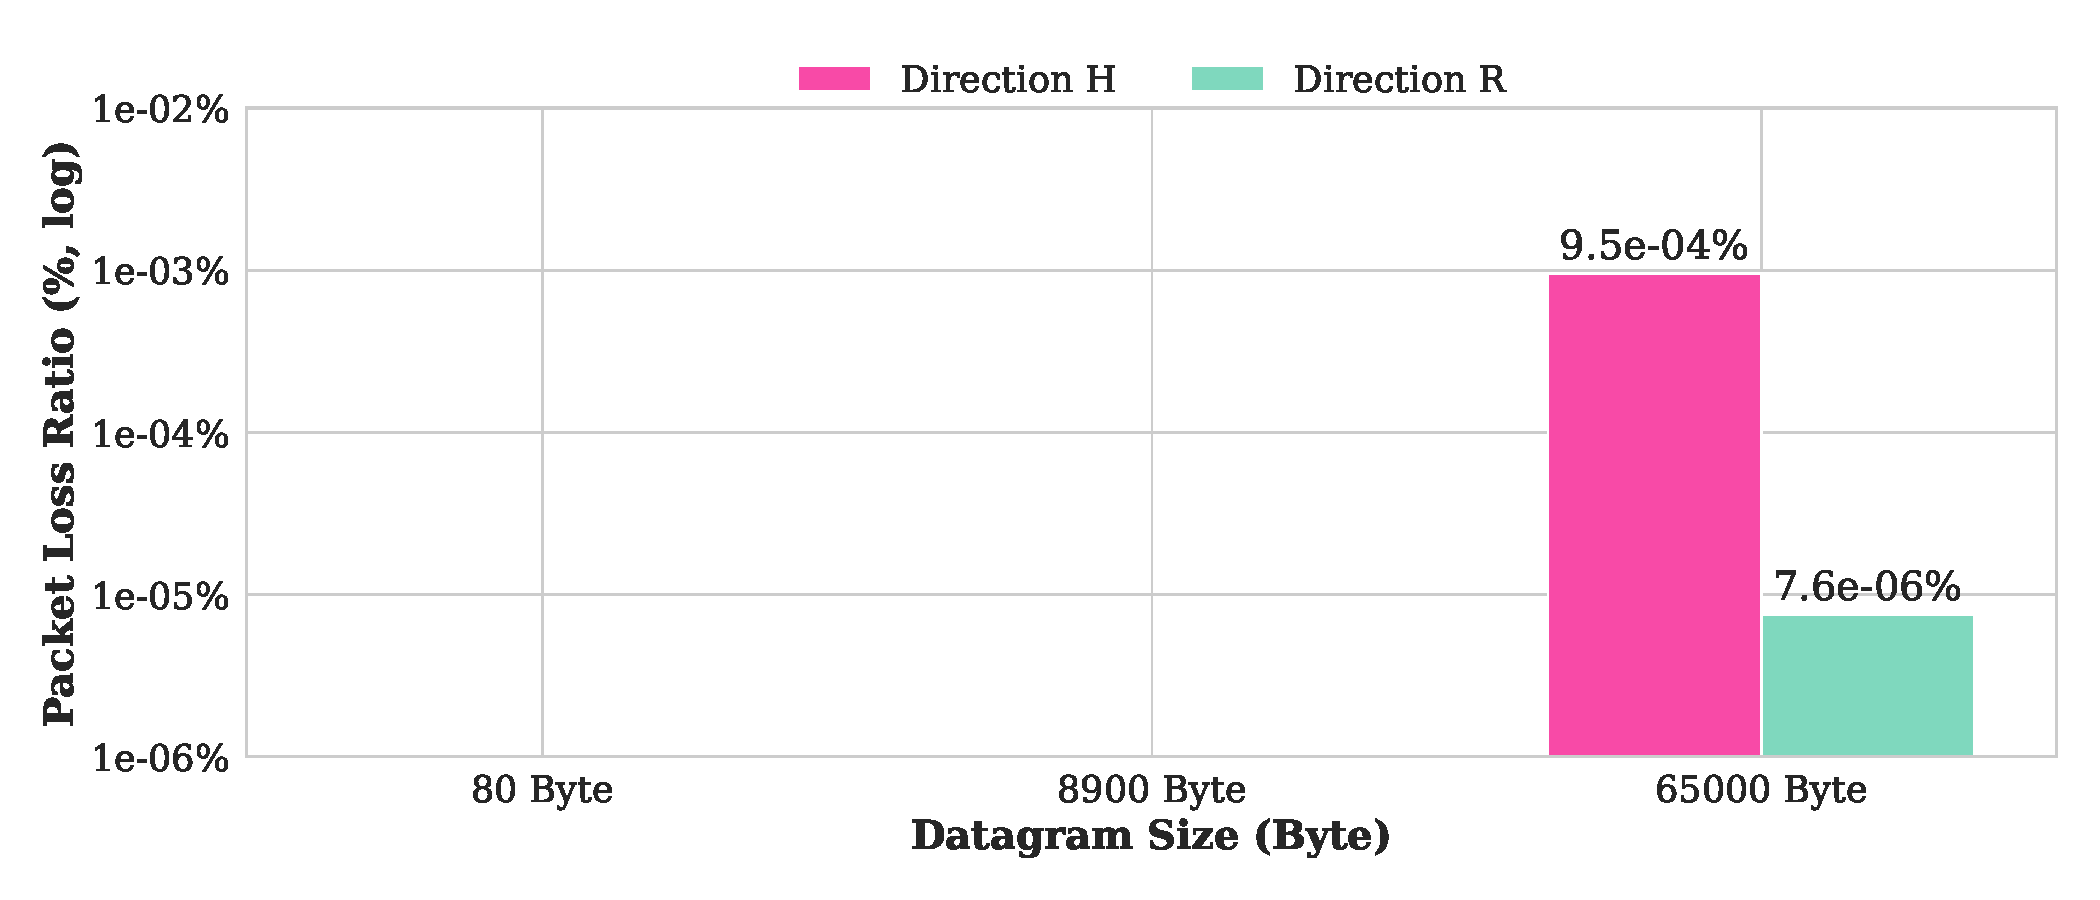
\includegraphics[width=1\linewidth]{figures/reliability/ihawk/diagr3.pdf}
    \caption{Packet Loss Ratio by Datagram Size and Communication Direction (Campaign `Tests without additional Load').}
    \label{fig:diagr3Loss}
\end{figure}

Figure \ref{fig:diagr3Loss} displays the overall packet loss ratio for this test campaign, categorized by datagram size and communication direction. No packet losses were observed during the tests conducted with datagram sizes of 80 and 8900 bytes. However, packet losses were observed in both the `H' and `R' directions during testing with a datagram size of 65000 bytes when using fragmented packets. Table \ref{tab:LossesC1} presents a breakdown of the losses by channel. The packet losses in the `H' and `R' directions will be analyzed separately separately below.

\begin{table}[h!]
\centering
\newcolumntype{C}[1]{>{\raggedright\arraybackslash}p{#1}}

\begin{subtable}{\linewidth}
\centering
\begin{tabular}{l| C{2.3cm} C{1.2cm} | l}
	\toprule
	\textbf{Channel} & \multicolumn{2}{l|}{\textbf{Lost Packets}} & \textbf{Average Throughput} \\
	\scriptsize{ }& \multicolumn{2}{l|}{\scriptsize{(Ratio/Total)}} & \scriptsize{ }\\
	\midrule
 	1A-H & \num{0} \% & / 0    & 9.90 GBit/s \\ 
 	1B-H & \num{0} \% & / 0    & 9.90 GBit/s \\
 	2A-H & \num{0} \% & / 0    & 9.89 GBit/s \\
 	2B-H & \num{0} \% & / 0    & 9.89 GBit/s \\
 	3A-H & \num{3.9e-03} \% & / 4313 & 9.89 GBit/s \\
 	3B-H & \num{3.8e-03} \% & / 4285 & 9.89 GBit/s \\
 	4A-H & \num{0} \% & / 0    & 9.90 GBit/s \\
 	4B-H & \num{0} \% & / 0    & 9.90 GBit/s \\
	\bottomrule
\end{tabular}
\caption{Direction `H'}
\label{tab:LossesC1:H}
\end{subtable}
\vspace{6pt}

\begin{subtable}{\linewidth}
\centering
\begin{tabular}{l|C{2.3cm} C{1.2cm}|l}
	\toprule
	\textbf{Channel} & \multicolumn{2}{l|}{\textbf{Lost Packets}} & \textbf{Average Throughput} \\
	\scriptsize{ }& \multicolumn{2}{l|}{\scriptsize{(Ratio/Total)}} & \scriptsize{ }\\
	\midrule
	1A-R & \num{5.0e-06} \% & / 7  & 8.25 GBit/s \\ 
 	1B-R & \num{9.1e-06} \% & / 11 & 8.75 GBit/s \\
	2A-R & \num{5.8e-06} \% & / 8  & 8.23 GBit/s \\
 	2B-R & \num{5.8e-06} \% & / 8  & 8.13 GBit/s \\
 	3A-R & \num{5.1e-06} \% & / 7  & 8.12 GBit/s \\
 	3B-R & \num{1.1e-05} \% & / 16 & 8.09 GBit/s \\
 	4A-R & \num{7.9e-06} \% & / 9  & 8.20 GBit/s \\
 	4B-R & \num{7.8e-06} \% & / 9  & 8.40 GBit/s \\
	\bottomrule
\end{tabular}
\caption{Direction `R'}
\label{tab:LossesC1:R}
\end{subtable}

\caption{Packet Losses and Average Throughput for a Datagram Size of 65000 Bytes (Campaign `Tests without additional Load').}
\label{tab:LossesC1}
\end{table}


Packet losses of \num{7.56e-6} \% were observed when examining a datagram size of 65000 bytes in the direction from the endpoints to the center (`R'). Table \ref{tab:LossesC1:R} provides a breakdown of these losses at a datagram size of 65000 bytes by channel, which shows that few losses occur in all communication channels in this direction and are almost evenly distributed among the individual channels.


\begin{figure}[h!]
    \centering
    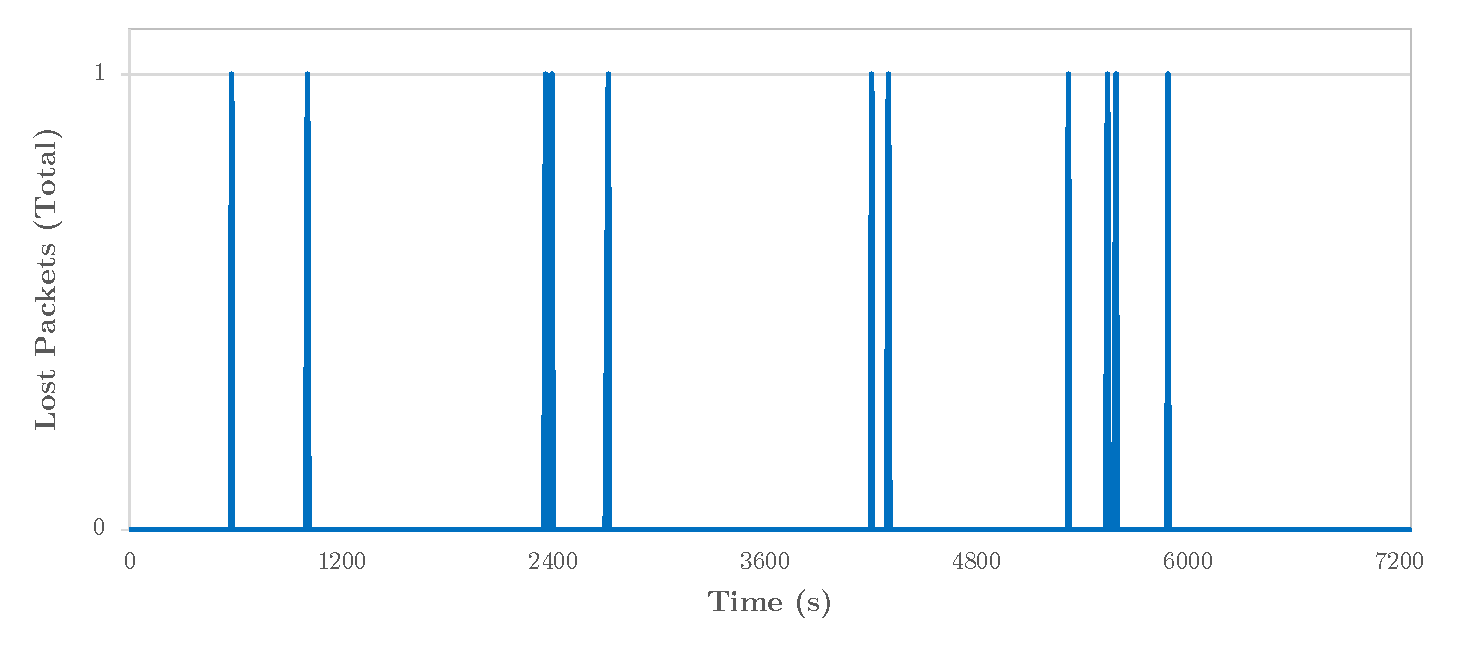
\includegraphics[width=1\linewidth]{figures/reliability/ihawk/diagr4.pdf}
    \caption{Temporal Distribution of Packet Loss for Channel 1B-R (Campaign `Tests without additional Load').}
    \label{fig:diagr4Temp}
\end{figure}

Figure \ref{fig:diagr4Temp} displays the temporal distribution of packet losses using channel 1B-R as an example. It is evident that the packet losses do not occur in bursts, but instead are distributed independently across the entire test duration. This trend can observed for the other channels.

Packet losses can occur at the sender (Endpoints in the `R' direction), during cable transmission on the route, or at the receiver (Center in the `R' direction). Further investigation is necessary to determine the precise location and reasons for packet losses, as the statistics of the network interfaces and the network stack on all computer systems for this direction do not indicate any drops.

To investigate the losses in the direction `R' at 65,000 bytes, test sessions of 20 minutes were run, gradually reducing the number of bidirectional links used until no losses occurred. The results of this investigation are displayed in Figure \ref{fig:diagr5Loss}.

\begin{figure}[h!]
    \centering
    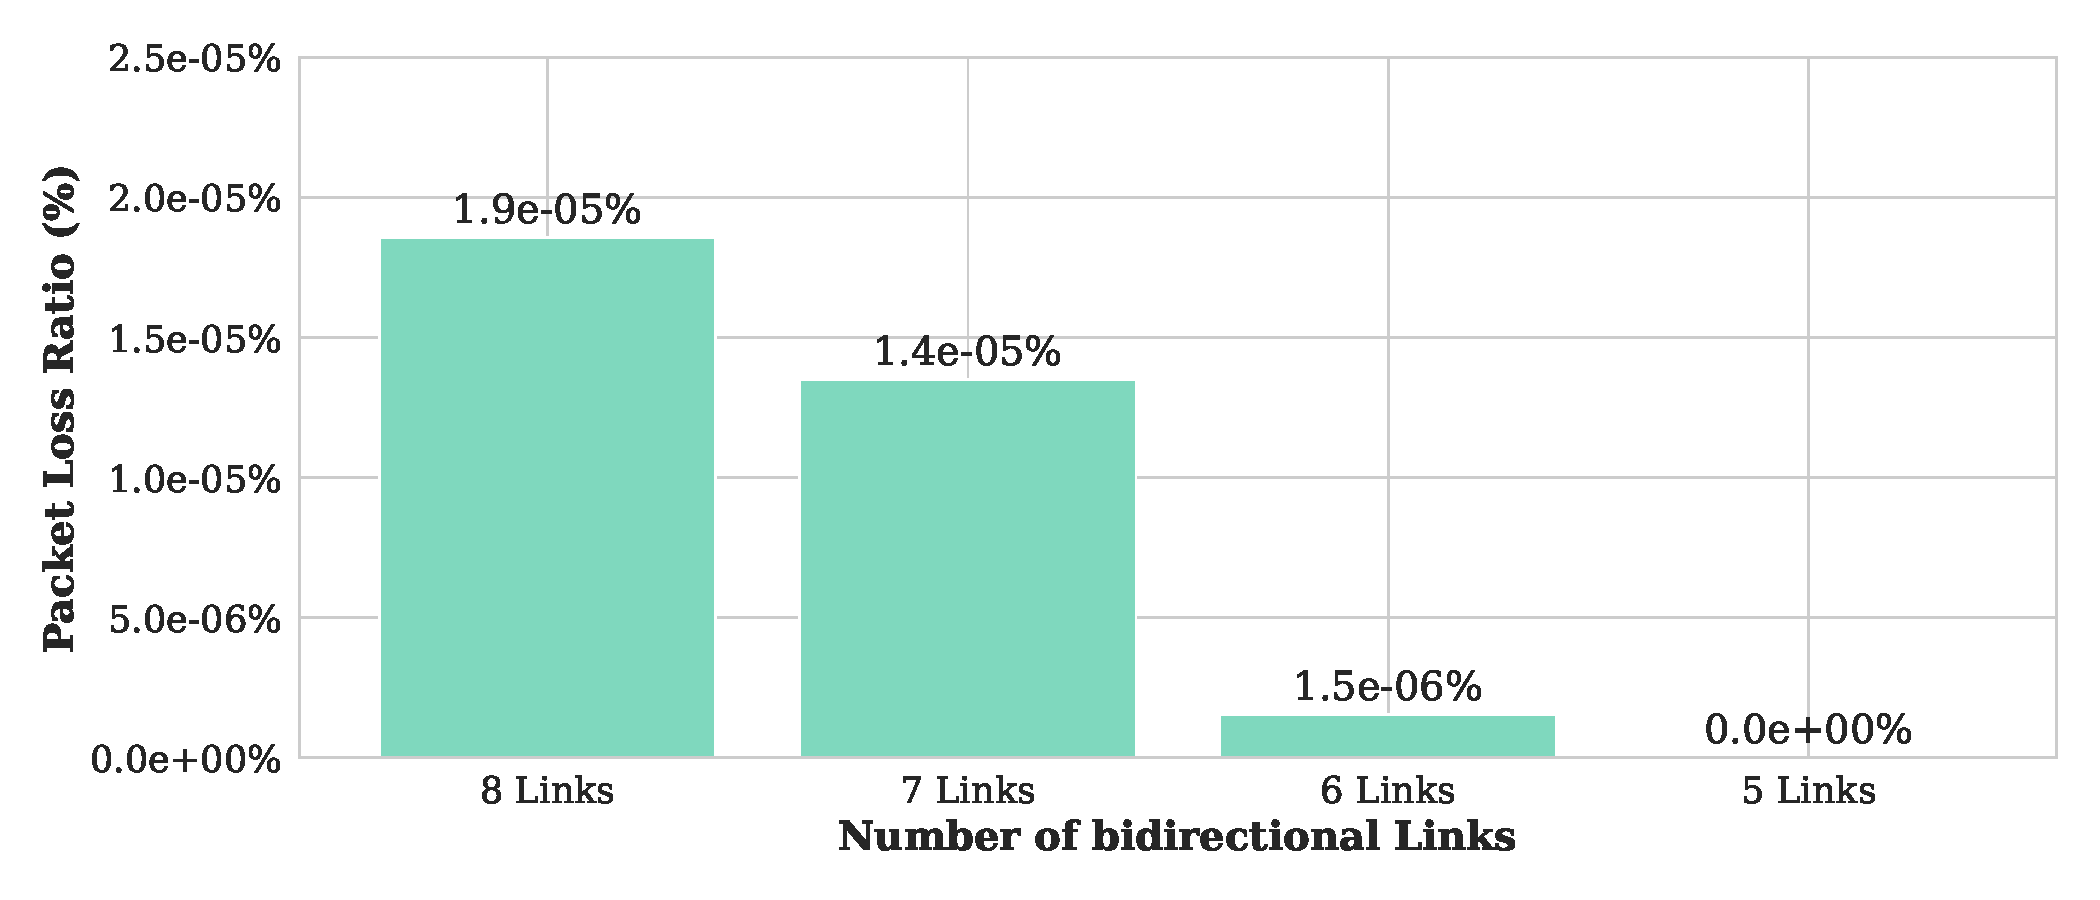
\includegraphics[width=1\linewidth]{figures/reliability/ihawk/diagr5.pdf}
    \caption{Packet Loss Ratio by Number of Links with a Datagram Size of 65000 Byte in Direction `R' (Campaign `Tests without additional Load').}
    \label{fig:diagr5Loss}
\end{figure}

The investigation shows that there are no losses in the direction `R' when using 5 bidirectional links. The ratio of losses to the total number of packets decreases as the number of links decreases.

In this test campaign, only the number of links decreased, but the configuration of the TestSuite remains unchanged. Therefore, the load on a single link remains the same, so the route cannot be considered the cause of the packet losses. In the test with five bidirectional links, endpoints 1 and 4 utilize both of their respective links, while endpoint 2 only utilizes link A. Endpoint 3 is not part of this test. Since the load on endpoints 1 and 4 is the same as in the original scenario with eight links, the senders, in this case the endpoints, are not considered to be responsible for the packet losses.

Based on these findings, it can be concluded that the receiver, in direction `R' the center, is where the packet losses occurred. Observing that losses occur only at a datagram size of 65000 bytes suggests a correlation with the defragmentation on the network stack. One possible scenario is an overflow of the buffer allocated for defragmentation, resulting in packet losses. \\


As displayed in figure \ref{fig:diagr3Loss}, the direction `H' from the center to endpoints experiences significantly higher packet loss at a rartio of \num{9.55e-4} \% for a datagram size of 65000 bytes compared to direction `R'. Table \ref{tab:LossesC1:H} includes a breakdown of the packet losses for a datagram size of 65000 bytes by channel. It is important to note that only packet losses were observed in communications with endpoint 3.

The statistics (Standard Interface Statistic and Network Stack Statistic) recorded in the sender (Center) show no losses. In contrast, the statistics for the affected receiver (Endpoint 3) show packet losses in the \texttt{rx\_missed\_errors} counter of the Standard Interface Statistic (see Table \ref{tab:ep3InterfaceStat}).

\begin{table}[h]
\centering
\begin{tabular}{l|l|l|l}
	\toprule
	\textbf{Interface} & \textbf{Channel} & \textbf{\texttt{rx\_dropped}} & \textbf{\texttt{rx\_missed\_errors}} \\
	\midrule
 	enp1s0f0 & 3A-(H/R) & 0 & 19507 \\ 
 	enp1s0f1 & 3B-(H/R) & 0 & 19414 \\
	\bottomrule
\end{tabular}
\caption{Extract of the Standard Interface Statistic for Endpoint 3.}
\label{tab:ep3InterfaceStat}
\end{table}

According to the Linux kernel documentation, \texttt{rx\_missed\_errors} indicates the number of packets that were dropped by the computer due to insufficient space in the buffer \cite{sock11}. This indicates that the computer may not be able to handle incoming packets at the rate at which they arrive at the network interface, resulting in network congestion at the endpoint 3. The ksoftriq threads, which handle the processing of incoming packets as described in \label{chap:recpath} were unable to process all the packets available in the network device's ring buffer before their CPU time expired.

The recorded losses of the TestSuite are lower than the values for \texttt{rx\_missed\_error}. This is due to the fact that losses only occurred at 65000 bytes, where the UDP packets were fragmented into 8 IP packets due to the configured MTU of 9000 bytes. If a fragment is lost, the entire packet is discarded.

\begin{figure}[h!]
    \centering
    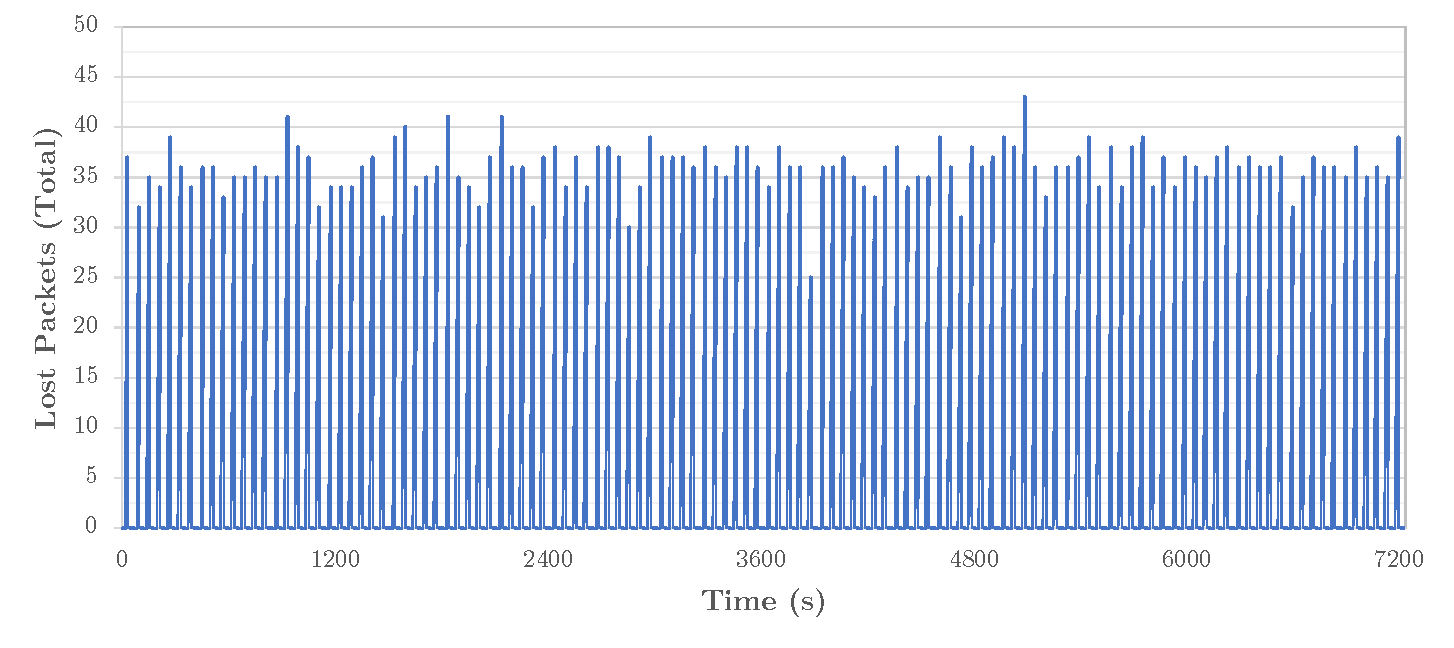
\includegraphics[width=1\linewidth]{figures/reliability/ihawk/diagr6.pdf}
    \caption{Temporal Distribution of Packet Loss for Channel 3A-H (Campaign `Tests without additional Load').}
    \label{fig:diagr6Temp}
\end{figure}

Figure 3 shows the temporal distribution of packet losses for communication 3A-H. The graph uses a resolution of 100,000 packets.  It is clear that packet losses occur uniformly over time rather than in bursts. Furthermore, it can be observed that losses are cyclic in nature. Upon examining the individual query requests, it is noticeable that there is a packet loss of approximately 30 to 40 packets every 900,000 packets (~65 seconds), but no packets are lost in the intervening period. The graph for 3B-H shows comparable results.

These results confirm the hypothesis of network congestion on endpoint 3, which where already assumed in the presentation of the standard interface statistics (see Table \ref{tab:ep3InterfaceStat}). However, there is no indication of CPU overload, as the average CPU utilization on endpoint 3 during this test was 36.7\%. An additional investigation focusing on endpoint 3 revealed no packet loss when using only one bidirectional link with this endpoint.

It is also important to note that packet losses are only observed on endpoint 3. Endpoint 2 and endpoint 3 belong to the Traffic PC system type (refer to \ref{chap:ComputerHardware}), meaning they utilize the same CPU and are equipped with the Intel X540-T2 network card. The recorded average CPU utilization of both computers during the test  was also almost identical.

The primary distinction between the two Traffic PCs is the motherboard. TPC1 (Endpoint 2) uses a GA-Z77X-UD5H motherboard, while TPC2 (Endpoint 3) is equipped with a GA-Z77X-UD3H motherboard. Although both motherboards have the PCIe x16 slot, which is used for the network card, connected directly to the CPU and feature the same Intel X77 chipset, there are still differences in the components and their cooling, which is more advanced on the GA-Z77X-UD5H \cite{reli04, reli05}.

Both computer systems are equipped with air cooling to provide heat dissipation to the CPU. However, TPC1 is equipped with a superior type of air cooling. As a result, the CPU of TPC2 may be subjected to higher temperatures compared to TPC1, which could lead to CPU throttling. This could be a possible explanation for the differences in packet loss observed between endpoints 2 and 3.

Table \ref{tab:LossesC1:H} shows that there were no losses observed in the `H' direction with the High-Performance PCs.

\paragraph{Classification of Results}

The results indicate that packet losses occur in the test setup when using all bidirectional links, both in the center and in endpoint 3 due to congestion. However, it should be noted that these losses are relatively modest and occur only at maximum load and only in conjunction with a datagram size of 65000 bytes with fragmentation.

\subsubsection{Tests with additional Load at the Center}

\paragraph{Motivation and Context}
The purpose of this test campaign is to analyze the reliability of the system under additional load at the center. The realistic scenario described in \ref{chap:campaignloadscen} was used as the additional system load. The number and intensity of stress-ng stressors on the computer system remain the same. However, no network stressors were used because the network load is entirely generated and measured by the TestSuite.

A test duration of 10 minutes was chosen. To maintain consistency with the prior campaign, datagrams sizes of 80, 8900, and 65000 bytes were tested. Despite packet loss in the previous scenario, a cycle time of 0 µs was again selected to evaluate the system under a high network load. All 16 communication channels were utilized.

\paragraph{Results}

\begin{figure}[h]
    \centering
    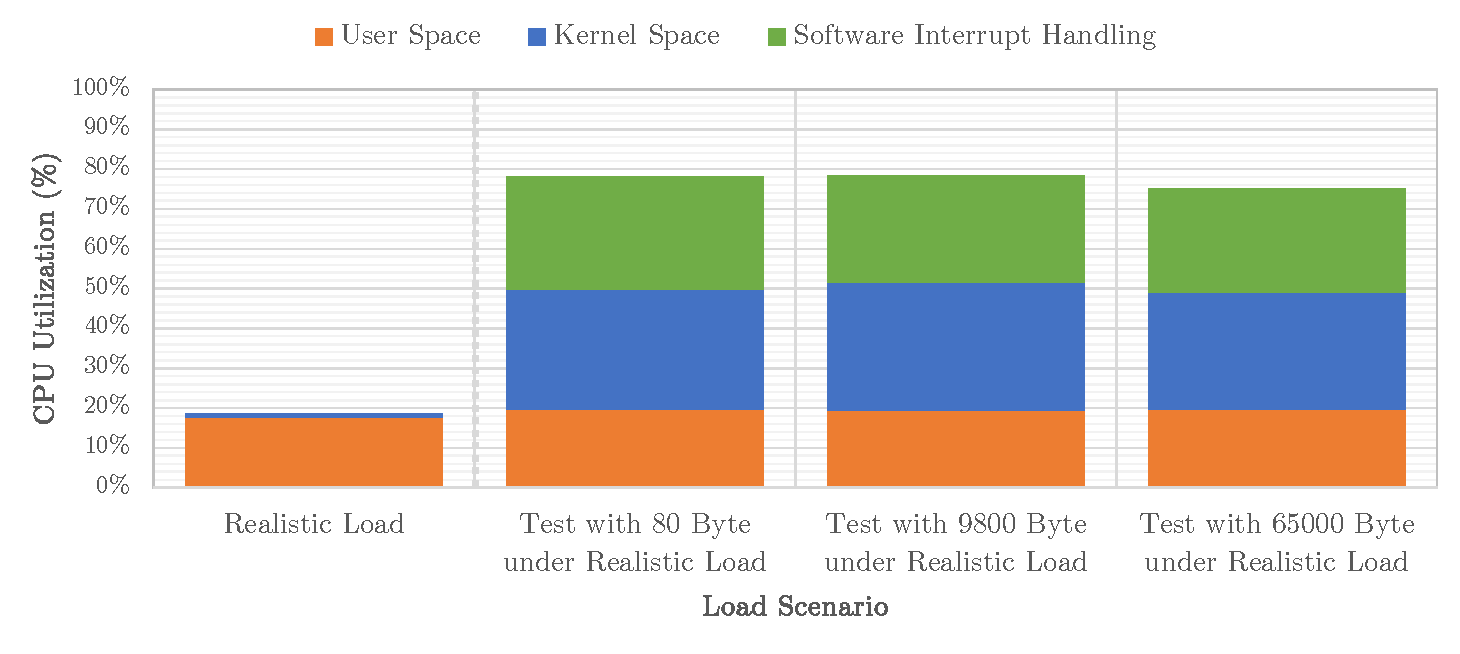
\includegraphics[width=1\linewidth]{figures/reliability/ihawk/diagr7.pdf}
    \caption{CPU Utilization in the Center for different Load Scenarios (Campaign `Tests with additional Load at the Center').}
    \label{fig:diagr7CPU}
\end{figure}

Figure \ref{fig:diagr7CPU} displays the average CPU utilization in the center during the execution of this test campaign and compares it with the execution of the realistic load scenario without running the tests with the TestSuite.

The realistic scenario utilizes 18.6\% of the CPU. The majority of the CPU time is spent in the user space with 17.6\% and 1\% is spent in the kernel space. The average CPU utilization during the execution of the test campaign is between 72\% and 78\%. No overload situation due to the additional system load can be identified when examining CPU utilization. Additionally, the transmission data transfer rate is also not affected by the additional load.

\begin{figure}[h]
    \centering
    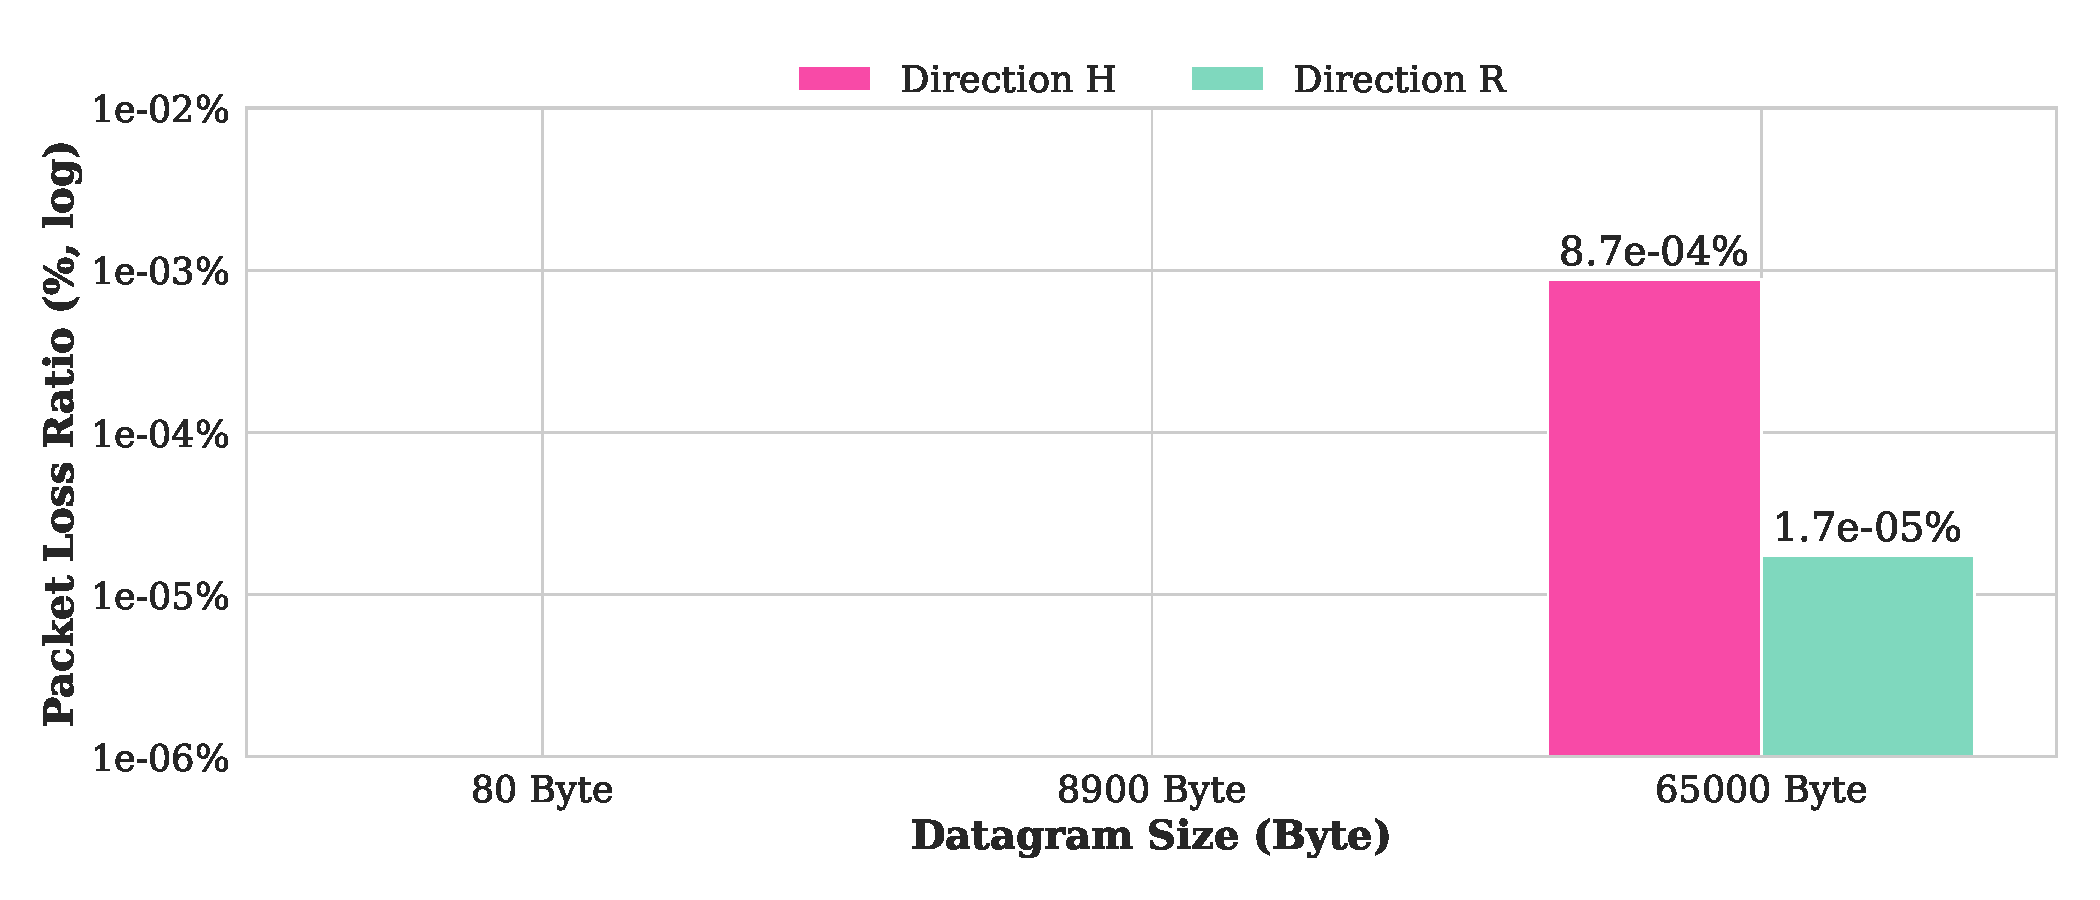
\includegraphics[width=1\linewidth]{figures/reliability/ihawk/diagr8.pdf}
    \caption{Packet Loss Ratio by Datagram Size and Communication Direction (Campaign `Tests with additional Load at the Center').}
    \label{fig:diagr8Loss}
\end{figure}

Figure \ref{fig:diagr8Loss} displays the results of the test campaign categorized by communication direction and datagram size. The results are consistent with those observed in the first test campaign (Figure \ref{fig:diagr3Loss}), as packet losses only occurred with a datagram size of 65000 bytes in both communication directions.

Packet losses were observed in the direction `H' (Center to Endpoints), which again only occurred during communication with endpoint 3. The reasons for those losses were already described in the previous section.

In direction `R' (Endpoints to Center), packet losses were also comparable to the results of the campaign without additional load. The loss ratio is with \num{1.75e-5} \% slightly higher than on the scenario without additional load (\num{7.56e-6} \%). A possible explanation for this might be a variation in the exact number of packet losses, as well as the shorter duration choosen for this campaign. The absolute number of these losses, however, is very low at 8 packets across all links in direction `R'.

\paragraph{Classification of Results}
The results of this campaign showed that the additional load on the iHawk in the center of the star had no impact on reliability, as the number of packet losses was comparable to the campaign with no additional load.


\subsubsection{Tests to Investigate the Influence of CPU Affinity} \label{chap:AffinityAnalysis}
\paragraph{Motivation and Context}

CPU affinity refers to the ability to bind processes to one or more specific CPU cores \cite{reli06}. The objective of this campaign is to examine the impact of various CPU affinity options applied to the center PC on the reliability.

As mentioned in \ref{chap:iHawkChar}, the iHawk's PCIe slots are directly connected to one of the CPUs. CPU 0 is connected to slots 1 to 3, which contain network cards connected to endpoints 2 and 3. Similarly, CPU 1 is connected to slots 4 to 6, which contain network cards connected to endpoints 1 and 4. The CPUs are interconnected through two UPI links. The purpose of the test campaign is to investigate any possible limitations in this two-socket configuration. These limitations could be caused by bottlenecks in the memory connection of the network cards and the connection between the CPUs.

If CPU affinity is not explicitly configured, the scheduler will assign arbitrary CPU cores to the corresponding TestSuite processes, as it has no information about which I/O devices are used by which process \cite{reli07}. In this test campaign, a scenario with 'enabled' CPU affinity was performed. This describes the situation when client and server processes of TestSuite were bound to the CPU cores on the local NUMA node. This refers to the CPU node to which the respective network card is connected. Additionally, a test was conducted usi`H'ng an 'inverse' CPU affinity, in which the processes of the TestSuite were configured to use CPU cores from the other socket. The Receive Side Scaling settings (see \ref{chap:ReceiveSideScaling}) of the network interface were not changed in all tests, as they are set by default to use only the cores on the local NUMA node.

Tests were performed with a duration of 10 minutes, using the same datagram sizes and a cycle time of 0 µs as in the previous campaigns.

\paragraph{Results}

\begin{figure}[h]
    \centering
    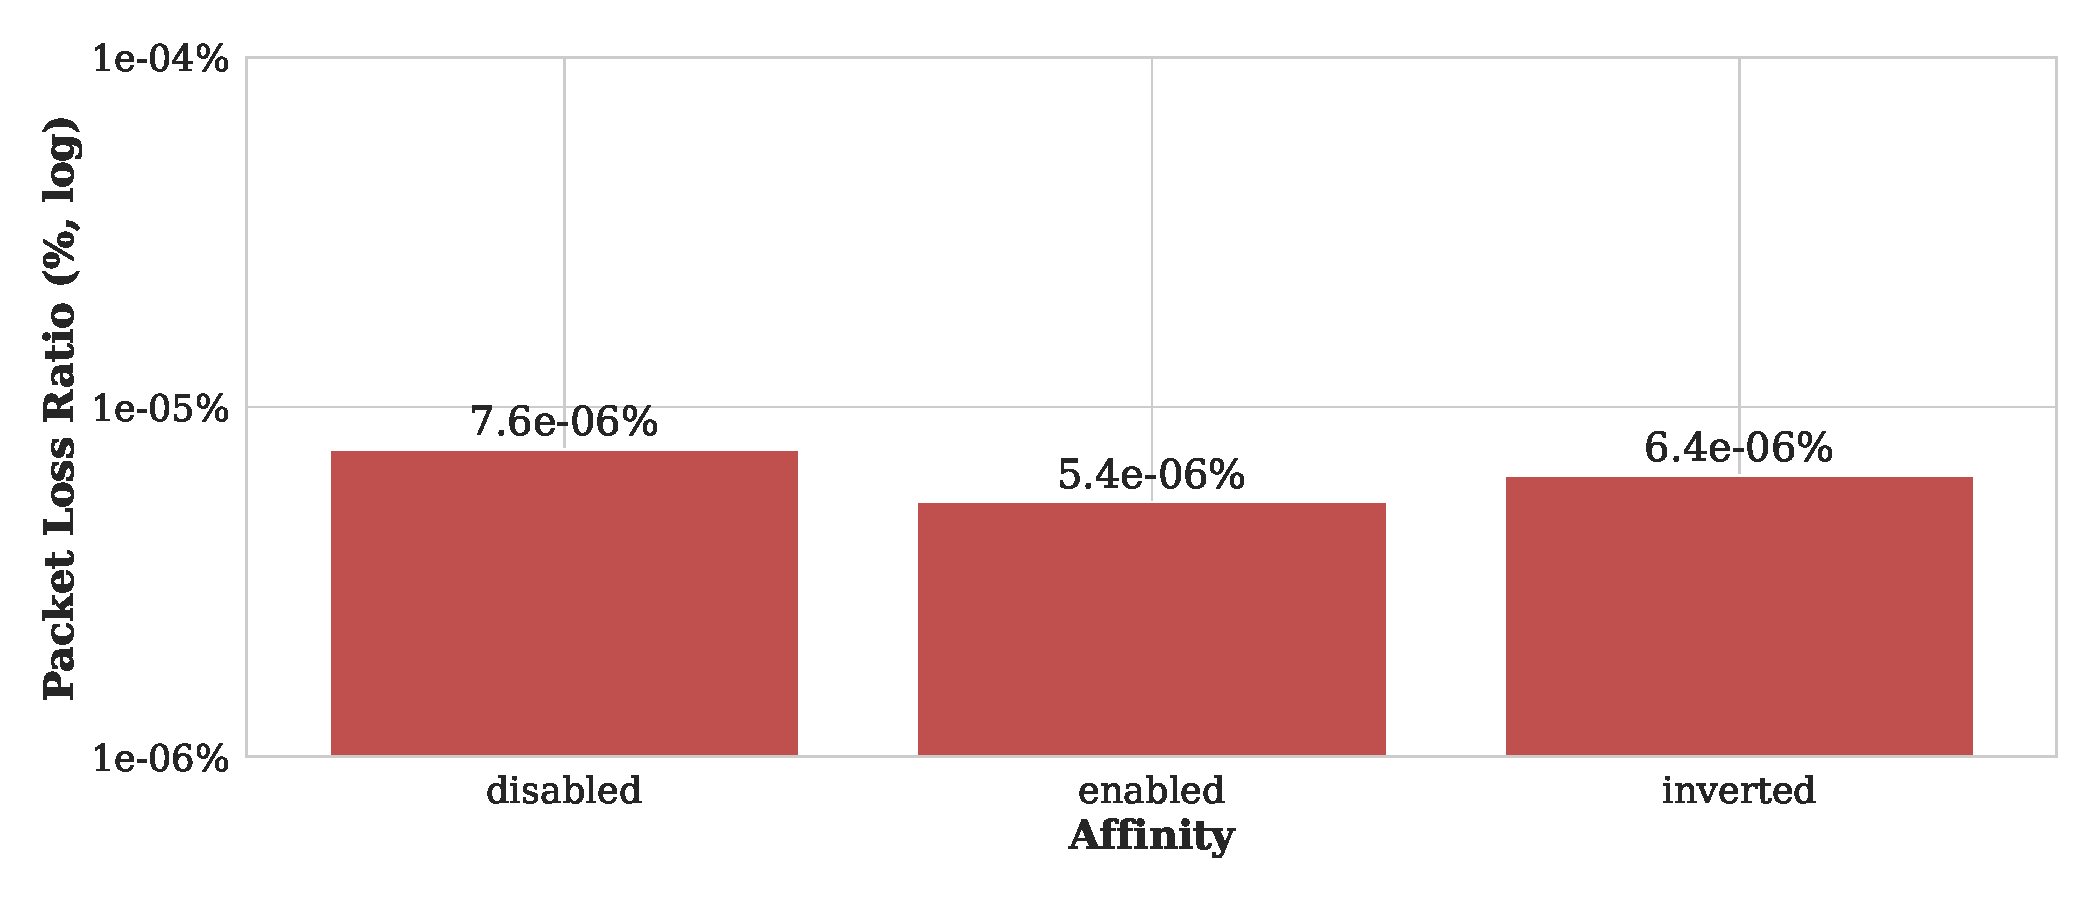
\includegraphics[width=1\linewidth]{figures/reliability/ihawk/diagr9.pdf}
    \caption{Packet Loss Ratio by Affinity Setting for a Datagram Size of 65000 Byte (Campaign `Tests to Investigate the Influence of CPU Affinity').}
    \label{fig:diagr9Loss}
\end{figure}

Figure \ref{fig:diagr9Loss} shows the packet losses using the two CPU affinity settings in the `R' direction (Endpoints to Center) for a datagram size of 65000 byte and compares them to the results with no affinity setting from a previous campaign. For all tests performed, packet losses were only detected with a datagram size of 65000 byte. The packet losses in the direction `H' (Center to Endpoints) will not be discussed in detail here, as no particular anomalies were observed compared to the other test campaigns. There were packet losses in the communication channels from the center to endpoint 3.

Packet losses were observed with all three affinity settings in direction `R' when the datagram size was 65000 bytes, which is in connection with fragmented packets. These losses were also observed in the previous test campaigns.  The packet loss ratio varies slightly depending on the affinity settings utilized, but remains within a comparable range, ranging from \num{7.6e-6} \%  to \num{5.4e-6} \%. These variations in individual tests result more from variations in the specific number of packet losses, combined with the relatively short duration of the tests, than from the different evaluated CPU affinity settings. The CPU utilization of the center is similar for all three CPU affinity choices being evaluated and have already been discussed in the 'Tests without additional Load' campaign (see \ref{chap:noaddloadTest}).

\begin{figure}[h]
    \centering
    \begin{subfigure}[b]{0.32\textwidth}
        \centering
        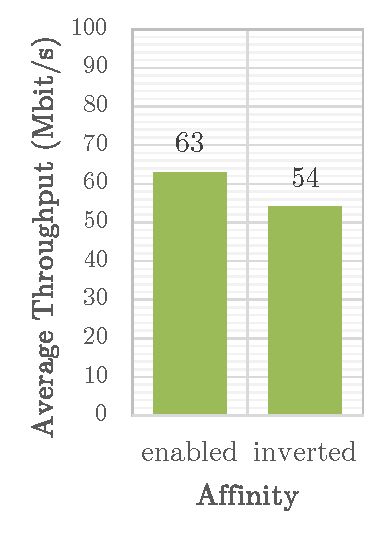
\includegraphics[width=\textwidth]{figures/reliability/ihawk/diagr10a.pdf}
        \caption{80 Byte}
    \end{subfigure}
    \hfill
    \begin{subfigure}[b]{0.32\textwidth}
        \centering
        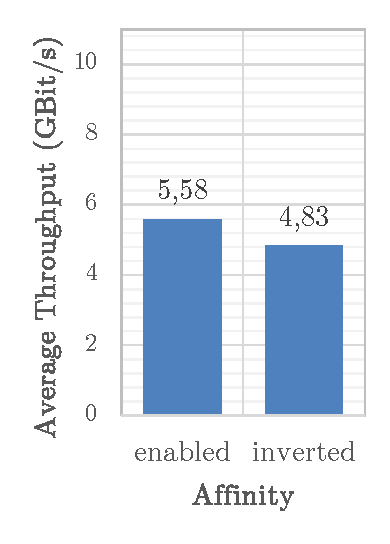
\includegraphics[width=\textwidth]{figures/reliability/ihawk/diagr10b.pdf}
        \caption{8900 Byte}
    \end{subfigure}
    \hfill
    \begin{subfigure}[b]{0.32\textwidth}
        \centering
        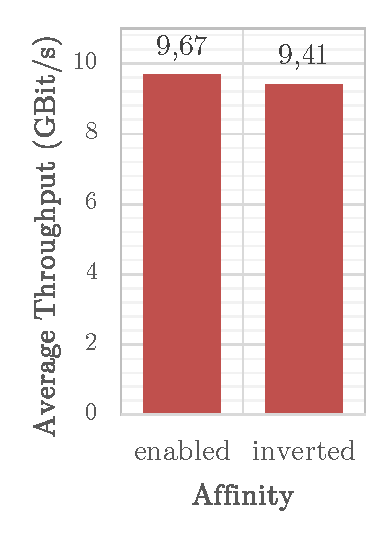
\includegraphics[width=\textwidth]{figures/reliability/ihawk/diagr10c.pdf}
        \caption{65000 Byte}
    \end{subfigure}
    \caption{Average Throughput for different Affinity Settings (Campaign `Tests to Investigate the Influence of CPU Affinity').}
    \label{fig:diagr10Throuhput}
\end{figure}

One notable result of this test campaign is the difference in the average transmit throughput of the center. Figure \ref{fig:diagr10Throuhput} compares the transmit data rates between 'enabled' and 'inverted' CPU affinity. The results show that, for datagram sizes of 80 bytes and 8900 bytes, the send throughput is approximately 15\% higher for the 'enabled' CPU affinity scenario than for the 'inverted' CPU affinity test. For a datagram size of 6500 bytes, the send throughput is approximately 3\% higher. The higher throughput is due to the fact that the CPU can access its local resources much faster than the other CPU. The UPI Link, which connects the two CPU sockets, has a latency of about 130 ns \cite{setup07}.

\paragraph{Classification of Results}
The results of this test campaign indicate that CPU affinity does not affect system reliability. Furthermore, it is important to note that potential bottlenecks in multi-socket systems, do not have an impact on the packet loss rate of a UDP communication.


\subsubsection{Tests to Investigate the Influence of Interrupt-Moderation} \label{chap:RelInterMod}
\paragraph{Motivation and Context}

Interrupt moderation, described in \ref{chap:InterMod}, can reduce the number of interrupts generated by the network interface.

This campaign investigates the influence of different settings for interrupt moderation on reliability. The reliability will be examined with deactivated interrupt moderation, as used in all previous campaigns. The recommended timeout values of 84 µs (equivaltent to \num{\sim{12000}} interrupts/s) and 62 µs (equivaltent to \num{\sim{16000}} interrupts/s) from the Intel Linux Performance Tuning Guide \cite{intermod03} were also tested. Additionally, adaptive interrupt moderation, which is active by default, was examined.  

The test campaign included tests with three datagram sizes of 80, 8900, and 65000 bytes, each with a duration of 5 minutes.

\paragraph{Results}
No significant differences in reliability were found among the various rates of interrupt moderation and the scenario without such moderation. Similar to the test scenario with interrupt moderation disabled, low levels of packet loss in direction `R' were detected in all three variants tested. Furthermore, packet losses were also detected at endpoint 3, as discussed in previous sections.

\begin{figure}[h]
    \centering
    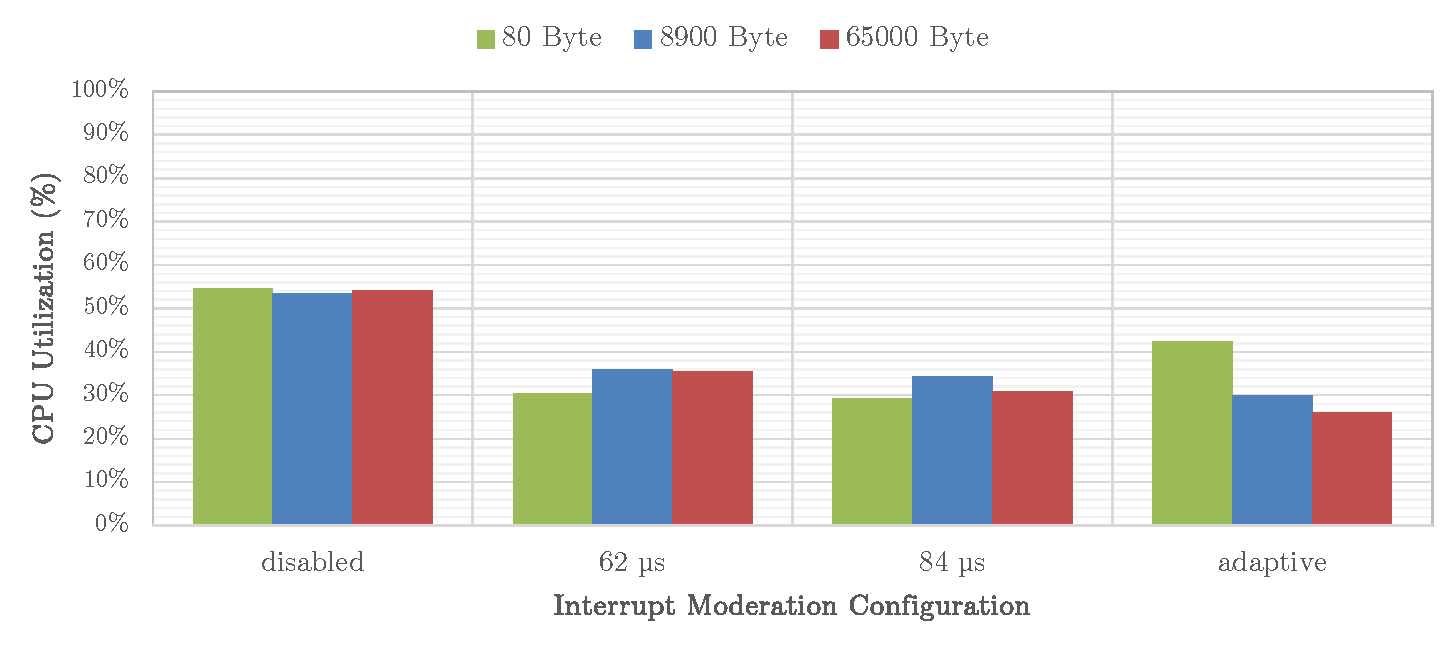
\includegraphics[width=1\linewidth]{figures/reliability/ihawk/diagr11.pdf}
    \caption{CPU Utilization in the Center for different Interrupt Moderation Configurations (Campaign `Tests to Investigate the Influence of Interrupt-Moderation').}
    \label{fig:diagr11CPU}
\end{figure}

Figure \ref{fig:diagr11CPU} displays CPU usage in the center with various interrupt moderation settings. As expected, the CPU usage reaches its maximum at about 54\% when interrupt moderation is disabled. All three datagram sizes exhibit similar values in this case. The two interrupt moderation rates of 84 µs and 62 µs record equally high CPU utilization rates of around 33\%, with slightly higher values observed for 62 µs. However, these two test scenarios revealed significant differences in datagram sizes across the various areas. When dealing with small datagrams, especially those of 80 byte in the test, a lower CPU utilization can be experienced. This is because a higher number of UDP packets per second are sent or received (\num{\sim{99000}} pps) compared to the other two datagram sizes (\num{\sim{81000}} pps for 8900 bytes and \num{\sim{19000}} pps for 65000 bytes). The utilization of interrupt moderation leads to a decrease in the number of interruptions generated and a reduction in CPU load.

Adaptive interrupt moderation demonstrated variations in CPU utilization between the examined datagram sizes when compared to a fixed moderation rate. In this case, the interrupt rate is adjusted to provide low latency or high throughput depending on the type of traffic. This process is explained in detail in the patent \cite{intermod04}. For small datagrams, a low interrupt moderation rate is selected, which is equivalent to a high number of interrupts per second. Conversely, for large datagrams, a high interrupt moderation rate is selected, which is equivalent to a lower number of interrupts per second. These results are consistent with the CPU usage, which is significantly higher for 80 bytes than for 8900 or 65000 bytes.

\paragraph{Classification of Results}
The campaign has shown that all examined interruption moderation rates exhibit comparable reliability. The differences in CPU utilization was also investigated.

Although adaptive interrupt moderation was found to be as reliable as other settings, it should not be used in the Distributed Test Support System at this time due to the uncontrollability of its implementation. While the function is described in \cite{intermod04}, the behavior of the implementation may be unpredictable if used without closer examination.

However, the interrupt moderation in connection with the selected interrupt rate also has an influence on the latency, which is considered in section 5. %TODO - Change Reference

\subsubsection{Tests with the Intel X540-T2 Network Interfaces in the Center} \label{chap:IntelRel540}
\paragraph{Motivation and Context}
This campaign investigates the reliability of the Intel X540-T2 network interface in the iHawk in the center of the star and compares it to the Intel X710-T2L network interface examined so far. Both interfaces are presented in \ref{chap:NicTypes} and have two RJ45 ports and are both 10 GbE capable. The X540 chipset network cards were released in 2012, which means they are 7 years older than the X710 chipset network cards, which were released in 2019 \cite{setupnw02, setupnw03}. In addition, interfaces use different drivers (see Table \ref{tab:drivernic}). Both devices offer comparable offloading mechanisms.

During testing, datagram sizes of 80 bytes, 8900 bytes, and 6500 bytes were considered with a cycle time of 0 µs and a test duration of 2 hours each.

\paragraph{Results}
The reliability results show no noticeable differences compared to the Intel X710-T2L network cards. In direction `R', a minimal number of packet losses were observed that can be attributed to the center, as previously mentioned. However, no packet losses were recorded in direction `H' during the test.

Moreover, there were no notable variations in the transmission data rates of the center achieved through the utilization of Intel X540-T2 network cards and those of Intel X710- T2L network cards. Both cards also show a similarly CPU utilization.

\paragraph{Classification of Results}
The results indicate that both network interfaces, the Intel X710-T2L and the Intel X540-T2, are suitable for use in the Distributed Test Support System from a reliability standpoint. 

\subsection{Insights}
Overall, packet losses were detected during the tests, but only under maximum load and in relation to fragmented packets with a size of 65,000 bytes. Therefore, although packet losses occurred, the investigated topology can still be considered suitable for a Distributed Test Support System.

No degradation was found with increased stress at the center or when changing the location of the CPU socket on which the send or receive process is executed. Additionally, no differences in reliability were found among the different interrupt moderation rates tested, despite a noticeable variation in CPU utilization.

The reliability of the Intel X540-T2 network card in the center was tested and no differences were found compared to the X710-T2L. Therefore, the Intel X540-T2 is also suitable for use in the center of a Distributed Test Support System.








